\documentclass[
	% -- opções da classe memoir --
	12pt,				% tamanho da fonte
	openany,			% capítulos começam em pág ímpar (insere página vazia caso preciso)
	oneside,
	%twoside,			% para impressão em recto e verso. Oposto a oneside
	a4paper,			% tamanho do papel. 
	% -- opções da classe abntex2 --
	%chapter=TITLE,		% títulos de capítulos convertidos em letras maiúsculas
	%section=TITLE,		% títulos de seções convertidos em letras maiúsculas
	%subsection=TITLE,	% títulos de subseções convertidos em letras maiúsculas
	%subsubsection=TITLE,% títulos de subsubseções convertidos em letras maiúsculas
	% -- opções do pacote babel --
	english,			% idioma adicional para hifenização
	spanish,			% idioma adicional para hifenização
	brazil				% o último idioma é o principal do documento
	]{ufscar}
	
\usepackage[utf8]{inputenc}
\usepackage{relsize}
\usepackage{lmodern}			% Usa a fonte Latin Modern		
\usepackage[T1]{fontenc}		% Selecao de codigos de fonte.
\usepackage{indentfirst}		% Indenta o primeiro parágrafo de cada seção.
\usepackage{color}				% Controle das cores
\usepackage{graphicx}			% Inclusão de gráficos
\usepackage{microtype} 			% para melhorias de justificação
\usepackage{pdfpages}
\usepackage{listings}

% ---
% Pacotes de citações
% ---
\usepackage[brazilian,hyperpageref]{backref}	 % Paginas com as citações na bibl
\usepackage[alf]{abntex2cite}	% Citações padrão ABNT

\usepackage{amsmath}
\usepackage{multirow}
\usepackage[flushleft]{threeparttable}
\usepackage{subcaption}
%\usepackage{graphicx}
\usepackage{lscape}
\usepackage{longtable}
\usepackage{tabularx}
\usepackage{array}
\usepackage[table]{xcolor}
%\usepackage[pdftex]{hyperref}
\usepackage{algpseudocode,algorithm}
\usepackage{longtable}
%\usepackage[page]{appendix}
\usepackage{emptypage}

%\usepackage[sectionbib]{bibunits}

% \renewcommand*{\cftchaptername}{CAPÍTULO\space}
 
\definecolor{lightgray2}{RGB}{238,238,238}

% --- 
% CONFIGURAÇÕES DE PACOTES
% --- 

% ---
% Configurações do pacote backref
% Usado sem a opção hyperpageref de backref
\renewcommand{\backrefpagesname}{Citado na(s) página(s):~}
% Texto padrão antes do número das páginas
\renewcommand{\backref}{}
% Define os textos da citação
\renewcommand*{\backrefalt}[4]{
	\ifcase #1 %
		Nenhuma citação no texto.%
	\or
		Citado na página #2.%
	\else
		Citado #1 vezes nas páginas #2.%
	\fi}%
% ---

\newcommand{\textnumero}{
    N\textsuperscript{\underline{o}}
}


% ---
% Informações de dados para CAPA e FOLHA DE ROSTO
% ---
\titulo{RELATÓRIO FINAL}
\autor{GABRIEL HENRIQUE PRZYTOCKI}
\local{CURITIBA}
\data{2021}
\orientador[Orientação]{JÚLIO CESAR NIEVOLA}
\instituicao{%
PONTIFÍCIA UNIVERSIDADE CATÓLICA DO PARANÁ
  \par
  PRÓ-REITORIA DE PESQUISA, PÓS-GRADUAÇÃO E INOVAÇÃO
PROGRAMA INSTITUCIONAL DE BOLSAS DE INICIAÇÃO CIENTÍFICA}
\tipotrabalho{Relatório Final}
% O preambulo deve conter o tipo do trabalho, o objetivo, 
% o nome da instituição e a área de concentração 
\preambulo{Relatório Final apresentado ao Programa Institucional de Bolsas de Iniciação Científica, Pró-Reitoria de Pesquisa e Pós-Graduação da Pontifícia Universidade Católica do Paraná, e órgãos de fomento, sob orientação do \textbf{Prof. Dr. Júlio Cesar Nievola}.}
% ---

% ---
% Configurações de aparência do PDF final

% alterando o aspecto da cor azul
\definecolor{blue}{RGB}{41,5,195}

% informações do PDF
\makeatletter
\hypersetup{
     	%pagebackref=true,
		pdftitle={\@title}, 
		pdfauthor={\@author},
    	pdfsubject={\imprimirpreambulo},
	    pdfcreator={LaTeX with abnTeX2},
		pdfkeywords={abnt}{latex}{abntex}{abntex2}{trabalho acadêmico}, 
		colorlinks=true,       		% false: boxed links; true: colored links
    	linkcolor=blue,          	% color of internal links
    	citecolor=blue,        		% color of links to bibliography
    	filecolor=magenta,      		% color of file links
		urlcolor=blue,
		bookmarksdepth=4
}
\makeatother
% --- 

% ---
% Posiciona figuras e tabelas no topo da página quando adicionadas sozinhas
% em um página em branco. Ver https://github.com/abntex/abntex2/issues/170
\makeatletter
\setlength{\@fptop}{5pt} % Set distance from top of page to first float
\makeatother
% ---

% ---
% Possibilita criação de Quadros e Lista de quadros.
% Ver https://github.com/abntex/abntex2/issues/176
%

% ---
% inserir lista de algoritmos
% ---
%\pdfbookmark[0]{\listalgorithmcfname}{loa}
%\makeatletter
%\renewcommand\numberline[1]{
    %Algoritmo \normalfont #1 – }
%\makeatother
%\listofalgorithms
%\cleardoublepage

%\makeatletter
%\def\numberline#1{\hb@xt@\@tempdima{#1\hfil}}
%\makeatother
% ---

%------LISTA DE ALGORITMOS---------------------------------------------
%\newcommand{\algoritmoname}{algoritmo}
%\newcommand{\listalgorithmcfname}{Lista de Algoritmos}

%\newlistof{listofalgoritmos}{loa}{\listalgorithmcfname}
%\renewcommand{\listalgorithmcfname}{Lista de Algoritmos}%
%\newlistentry{algoritmo}{loa}{0}


% configurações para atender às regras da ABNT
%\setfloatadjustment{algoritmo}{\centering}
%\counterwithout{algoritmo}{section}
%\renewcommand{\cftalgoritmoname}{\algoritmoname\newline} 
%\renewcommand*{\cftalgoritmoaftersnum}{\hfill--\hfill}

\makeatletter
\def\numberline#1{\hb@xt@\@tempdima{#1\hfil}}
\makeatother

%\setfloatlocations{algoritmo}{hbtp} % Ver https://github.com/abntex/abntex2/issues/176
% ---

% --- 
% Espaçamentos entre linhas e parágrafos 
% --- 

% O tamanho do parágrafo é dado por:
\setlength{\parindent}{1.3cm}

% Controle do espaçamento entre um parágrafo e outro:
\setlength{\parskip}{0.2cm}  % tente também \onelineskip

% ---
% compila o indice
% ---
\makeindex
% ---

% Lista de simbolos
\makeatletter

\newcommand{\simbolo}[2]{\addcontentsline{lsb}{simb}{\numberline{#1}{#2}}}

\newcommand{\l@simb}[2]{
	\vskip -0.5cm
	\leftskip 0.0cm
	\parfillskip -\rightskip
	\parindent 0cm
	\@tempdima 2.5cm
	\advance\leftskip \@tempdima \null\nobreak\hskip -\leftskip
	{\normalfont {#1}}\nobreak \filltocentry{#2}
}

\newcommand{\imprimirlistadesimbolos}
{
	\pretextualchapter{\listadesimbolosname}\@starttoc{lsb}
	\cleardoublepage
}

\makeatother
% Fim lista de simbolos

% Lista de abreviacoes
% 
\newcommand{\imprimirlistadesiglas}{%
	    \pdfbookmark[0]{\listadesiglasname}{acn}	
		\printacronyms[%
				style=mylong1,
				title={\listadesiglasname \vspace{-0.2cm}}  % A lista de siglas ainda fica com um espaço a mais
			  ]
		\cleardoublepage
}
% Fim lista de abreviacoes

\usepackage[brazil]{babel}
\addto\captionsbrazil{\renewcommand{\listfigurename}{Lista de Figuras}}
\addto\captionsbrazil{\renewcommand{\listtablename}{Lista de Tabelas}}
\addto\captionsbrazil{\renewcommand{\listadesimbolosname}{Lista de Símbolos}}
\addto\captionsbrazil{\renewcommand{\listadesiglasname}{Lista de Abreviações}}
%\addto\captionsbrazil{\renewcommand{\listofalgorithms}{Lista de Algoritmos}}

\usepackage{listings}
\usepackage{xcolor}

\definecolor{corComentario}{RGB}{150,150,150}
\definecolor{corString}{RGB}{206,123,0}
\definecolor{corPalavraChave}{RGB}{0,0,230}
\definecolor{codegray}{rgb}{0.5,0.5,0.5}

\lstset{
	numbers=left,
	stepnumber=1,
	firstnumber=1,
	numberstyle=\tiny\color{codegray},
	extendedchars=true,
	breaklines=true,
	lineskip=0pt,
	frame=tb,
	basicstyle=\ttfamily\scriptsize,
	showstringspaces=false,
	stringstyle=\color{corString},
	commentstyle=\color{corComentario},
	keywordstyle=\color{corPalavraChave}
}

%\lstset{style=mystyle}

\setlength\extrarowheight{7pt}


\renewcommand{\listalgorithmname}{Lista de Algoritmos}


% -------------------------------------------------------------------------------------------------
% Início do documento
% -------------------------------------------------------------------------------------------------


\begin{document}

\frontmatter

\renewcommand{\listfigurename}{Lista de Figuras}
\renewcommand{\listtablename}{Lista de Tabelas}
\renewcommand{\listadesimbolosname}{Lista de Símbolos}
\renewcommand{\listadesiglasname}{Lista de Abreviações}
%\renewcommand{\listofalgorithms}{Lista de Algoritmos}

% Seleciona o idioma do documento (conforme pacotes do babel)
%\selectlanguage{english}
\selectlanguage{brazil}

% Retira espaço extra obsoleto entre as frases.
\frenchspacing 

% Declaracoes em Português
\algrenewcommand\algorithmicend{\textbf{fim}}
\algrenewcommand\algorithmicdo{\textbf{faça}}
\algrenewcommand\algorithmicwhile{\textbf{enquanto}}
\algrenewcommand\algorithmicfor{\textbf{para}}
\algrenewcommand\algorithmicif{\textbf{se}}
\algrenewcommand\algorithmicthen{\textbf{então}}
\algrenewcommand\algorithmicelse{\textbf{senão}}
\algrenewcommand\algorithmicreturn{\textbf{devolve}}
\algrenewcommand\algorithmicfunction{\textbf{função}}

% Rearranja os finais de cada estrutura
\algrenewtext{EndWhile}{\algorithmicend\ \algorithmicwhile}
\algrenewtext{EndFor}{\algorithmicend\ \algorithmicfor}
\algrenewtext{EndIf}{\algorithmicend\ \algorithmicif}
\algrenewtext{EndFunction}{\algorithmicend\ \algorithmicfunction}

% O comando For, a seguir, retorna 'para #1 -- #2 até #3 faça'
\algnewcommand\algorithmicto{\textbf{até}}
\algrenewtext{For}[3]%
{\algorithmicfor\ #1 $\gets$ #2 \algorithmicto\ #3 \algorithmicdo}

% ----------------------------------------------------------
% ELEMENTOS PRÉ-TEXTUAIS
% ----------------------------------------------------------
% \pretextual

% ---
% Capa
% ---
\imprimircapa
% ---

% ---
% Folha de rosto
% (o * indica que haverá a ficha bibliográfica)
% ---
\imprimirfolhaderosto*
% ---

% ---
% Inserir a ficha bibliografica
% ---

% Isto é um exemplo de Ficha Catalográfica, ou ``Dados internacionais de
% catalogação-na-publicação''. Você pode utilizar este modelo como referência. 
% Porém, provavelmente a biblioteca da sua universidade lhe fornecerá um PDF
% com a ficha catalográfica definitiva após a defesa do trabalho. Quando estiver
% com o documento, salve-o como PDF no diretório do seu projeto e substitua todo
% o conteúdo de implementação deste arquivo pelo comando abaixo:
%
% \begin{fichacatalografica}
%     \includepdf{fig_ficha_catalografica.pdf}
% \end{fichacatalografica}

\begin{fichacatalografica}

%%%%%%%%%%%%%%%% ATENCAO %%%%%%%%%%%%%%%%%%%%%%%
% Apos gerar ficha catalografica remove comentário a linha abaixo e fazer upload do arquivo ficha_catalografica.pdf %	

%\includepdf{ficha_catalografica.pdf}

\end{fichacatalografica}
% ---

% ---

% ---
% Inserir folha de aprovação
% ---

% Isto é um exemplo de Folha de aprovação, elemento obrigatório da NBR
% 14724/2011 (seção 4.2.1.3). Você pode utilizar este modelo até a aprovação
% do trabalho. Após isso, substitua todo o conteúdo deste arquivo por uma
% imagem da página assinada pela banca com o comando abaixo:
%
% \begin{folhadeaprovacao}
% \includepdf{folhadeaprovacao_final.pdf}
% \end{folhadeaprovacao}
%
\begin{folhadeaprovacao}

%%%%%%%%%%%%%%%% ATENCAO %%%%%%%%%%%%%%%%%%%%%%%
%Remover comentario da linha abaixo e fazer upload do arquivo folha-de-aprovacao.pdf %	

% \includepdf{folha-de-aprovacao.pdf}
  
\end{folhadeaprovacao}
% ---

% ---
% Dedicatória
% ---
%\begin{dedicatoria}
   %\vspace*{\fill}
   %\centering
   %\noindent
   %\textit{ Dedico este trabalho a todos os alunos de pós-graduação da UFSCar que queiram utilizar o LaTex.} \vspace*{\fill}
%\end{dedicatoria}
% ---

% ---
% Agradecimentos
% ---
%\begin{agradecimentos}
%Agradecimentos

%\end{agradecimentos}

%CAPES
%O presente trabalho foi realizado com apoio da Coordenação de Aperfeiçoamento de Pessoal de Nível Superior - Brasil (CAPES) - Código de Financiamento 001

% ---

% ---
% Epígrafe
% ---
%\begin{epigrafe}
    %\vspace*{\fill}
	%\begin{flushright}
		%\textit{``Toda a obra de um homem, seja em literatura, música, pintura, arquitetura ou em qualquer outra coisa, é sempre um auto-retrato; e quanto mais ele se tentar esconder, mais o seu caráter se revelará, contra a sua vontade.\\
		%(Samuel Butler)}
	%\end{flushright}
%\end{epigrafe}
% ---

\pagenumbering{roman}

% ---
% inserir lista de ilustrações
% ---
\pdfbookmark[0]{\listfigurename}{lof}
\setcounter{page}{3}
\addcontentsline{toc}{section}{LISTA DE FIGURAS}

\listoffigures*
\cleardoublepage
% ---

% ---
% inserir lista de tabelas
% ---
\pdfbookmark[0]{\listtablename}{lot}
\setcounter{page}{4}
\addcontentsline{toc}{section}{LISTA DE TABELAS}

\listoftables*
\cleardoublepage
% ---

% ---
% inserir lista de algoritmos
% ---
%\newfloat[section]{algoritmo}{loa}{\listofalgoritmosname}
% ---
% inserir lista de algoritmos
% ---
%\pdfbookmark[0]{\listalgorithmcfname}{loa}
\addcontentsline{toc}{section}{LISTA DE ALGORITMOS}
%\renewcommand{\listalgorithmcfname}{Lista de Algoritmos}%
%\makeatletter
%\renewcommand\numberline[1]{
    %Algoritmo \normalfont #1 – }
%\makeatother
%\renewcommand{\listalgorithmcfname}{List of Algorithmus}
\listofalgorithms
\setcounter{page}{5}
\cleardoublepage

\makeatletter
\def\numberline#1{\hb@xt@\@tempdima{#1\hfil}}
\makeatother
% ---
%\pdfbookmark[0]{\listofalgoritmosname}{loa}
%\listofalgoritmos*
%\cleardoublepage
% ---

% Lista de simbolos
\begin{simbolos}
\setcounter{page}{6}
\addcontentsline{toc}{section}{LISTA DE SÍMBOLOS}
\item[$ \vec{p_c} $] \textit{array com preços de fechamento de uma determinada ação}
\item[$ \vec{p_p} $] \textit{array com preços previstos por algum modelo para os fechamentos de uma ação}
\item[$ c $] \textit{carteira inicial para uma operação de trading}
\item[$ k $] \textit{constante do modelo Autorregressivo}
\item[$ \varepsilon $] \textit{ruído branco}
\item[$ \theta $] \textit{valor observado}
\item[$ \hat{\theta} $] \textit{valor estimado}
\end{simbolos}
% Fim lista de simbolos

% Lista de abreviações
\begin{siglas}
\setcounter{page}{7}
\addcontentsline{toc}{section}{LISTA DE ABREVIAÇÕES}
\item[AR] \textit{Acurácia das Operações com Lucro}
\item[AOL] \textit{Convolutional Neural Network - Rede Neural Convolucional}
\item[CI] \textit{Carteira Inicial}
\item[CF] \textit{Carteira Final}
\item[ET] \textit{Estratégia de Trading}
\item[FP] \textit{False Positive - Falso Positivo}
\item[FN] \textit{False Negative - Falso Negativo}
\item[LSTM] \textit{Long Short-Term Memory}
\item[MSE] \textit{Mean Squared Error - Erro quadrático médio}
\item[QAC] \textit{Quantidade de Ações Compradas}
\item[RC] \textit{Razão entre as Carteiras}
\item[RMT] \textit{Real Movements Trading}
\item[TP] \textit{True Positive - Verdadeiro Positivo}
\item[TN] \textit{True Negative - Verdadeiro Negativo}
\end{siglas}
% Fim lista de abreviações


\newcommand{\listappendicesname}{ANEXOS}
\newlistof{appendices}{apc}{\listappendicesname}
\newcommand{\appendices}[1]{\addcontentsline{apc}{appendices}{#1}}


%\listoffigures*
\cleardoublepage


% ---
% inserir o sumario
% ---
\pdfbookmark[0]{\contentsname}{toc}
\addcontentsline{toc}{section}{SUMÁRIO}
\tableofcontents*
%\mainmatter
\cleardoublepage
% ---

% RESUMO
% resumo em português
\setlength{\absparsep}{18pt} % ajusta o espaçamento dos parágrafos do resumo
\begin{resumo}
\addcontentsline{toc}{section}{RESUMO}
A previsão de movimentos no mercado de ações é uma tarefa complexa, apresentando inúmeras abordagens que objetivam uma maximização dos lucros em contrapartida de uma minimização das perdas e dos riscos por parte dos investidores. As técnicas mais recentes de redes neurais (CNN e LSTM), apesar de seu ótimo desempenho em inúmeras áreas, contrastam com a ausência de trabalhos voltados para sua utilização no mercado de ações. Este trabalho buscou comparar tais técnicas com o modelo Autorregressivo, clássico na previsão em séries temporais, bem como a modelos mais simples e ``ingênuos'' de previsão, de maneira a ter uma base maior de discussão. Os modelos foram testados com as ações PETR4.SA (Petrobrás) para os anos 2019 e 2020, oscilando em períodos diferentes de treino e teste, bem como repetindo os experimentos para uma maior assertividade dos resultados. As previsões geradas pelos modelos foram ainda submetidas à operações de \textit{trading} nos períodos de teste, utilizando classificações de ``alta'' e ``baixa'' em relação ao preço de fechamento do dia seguinte na tomada de decisão. Os rótulos dos movimentos foram gerados através de um algoritmo específico que separava em uma das duas classes os preços numéricos obtidos pelos modelos. Os resultados apontaram que a técnica CNN apresentou um desempenho aproximado em relação ao modelo Autorregressivo em termos de acurácia de operações com lucro (60\%), bem como +73\% desta acurácia em relação ao \textit{Naive Model} (Modelo Ingênuo) e +20\% em relação ao algoritmo de investimento \textit{Naive Trading} (Trading Ingênuo, utilizando apenas os preços dos dois dias anteriores para a tomada de decisão). Os experimentos realizados nas condições específicas deste trabalho, em termos dos parâmetros utilizados e o período da ação em questão, demostraram que o LSTM teve um desempenho ineficaz no que diz respeito às classificações dos movimentos e operação de \textit{trading}, bem como um desempenho comparável ao modelo autorregressivo em termos de previsões numéricas, considerando a proximidade como o valor real de fechamento. A técnica CNN foi especialmente eficiente para os propósitos deste trabalho, tal como é ressaltado na bibliografia consultada em relação ao seu uso para predição em séries temporais.

 \textbf{Palavras-chave}: \textit{Deep Learning}, CNN, LSTM, Mercado de Ações, Séries Temporais.
 
\end{resumo}

% ELEMENTOS TEXTUAIS
\textual

% Capitulo 1 - Introdução
\chapter{Introdução}

\pagenumbering{arabic}
\setcounter{page}{11}

\par
A previsão de movimentos do mercado financeiro é objeto de estudo de inúmeras abordagens, historicamente se adaptando para elevar ao máximo a precisão de seus modelos preditivos e inevitavelmente culminando na instrumentalização da tecnologia para o processamento e implementação de técnicas cada vez mais completas e precisas, diante da volatidade e o volume massivo de dados característicos deste mercado. \cite{senDattaChau2015}.

\par
Consequentemente, é evidente o crescimento da abordagem baseada nas Técnicas de Aprendizagem de Máquina (“\textit{Machine Learning}”) no que tange à análise de \textbf{Séries Temporais Financeiras}, especificamente mencionando as técnicas de \textit{Deep Learning}, notoriamente expressivas nos últimos cinco anos\footnote[1]{Disponível em: \href{https://scholar.google.com.br/scholar?q=\%22CNN\%22+\%22LSTM\%22+\%22bolsa+de+valores\%22\&hl=pt-BR\&as\_sdt=0\%2C5\&as\_ylo=2000\&as\_yhi=2021}{Google Acadêmico}. Acesso em 30 jan. 2021.}. Tais abordagens relacionadas à Séries Temporais Financeiras partem da análise do histórico passado de uma ação, e ações similares, realizando assim aproximações acerca de seu comportamento futuro; os padrões extraídos usualmente são combinados a técnicas específicas de mineração de dados, tais como associação, agrupamento, classificação, sumarização e regressão \cite{fu2011}. As Séries Temporais Financeiras são um subcampo de estudo de uma área matemática e estatística denominada de Séries Temporais, como é o caso das Séries provenientes da bolsa de valores: essencialmente dinâmicas, não lineares, complexas, não paramétricas e caóticas \cite{abuMostafaAtiya96}.

\par
Considerando a motivação dos investidores ao elaborar uma carteira, objetiva-se obter lucro máximo, em contrapartida de um risco mínimo; assim, torna-se evidente a problemática aqui destacada: diante da complexidade do problema, quais são as melhores formas de se utilizar as técnicas atuais de \textit{Deep Learning} na \textbf{classificação} e predição dos movimentos futuros da Bolsa de Valores? Em decorrência dos fatores acima mencionados, a emergência da nova abordagem, especialmente no que se refere às técnicas de \textit{Deep Learning}, considerando sua eficácia em inúmeros campos, contrastam com a ausência de trabalhos que busquem avaliar seu desempenho e identificar situações potenciais de uso, justificando assim a análise e avaliação a serem feitas nesse trabalho.

% Capitulo 2 - Objetivos
\chapter{Objetivos}

\par
Avaliar o desempenho de algoritmos de \textit{Deep Learning} (CNN e LSTM), classificando o movimento de uma ação para o dia seguinte em “crescente” ou “decrescente”, simulando operações de compra e venda de ações a fim de avaliar seus desempenhos.

\subsection{Objetivos específicos}
\begin{itemize}
\item Determinar o conjunto de atributos a serem utilizados para previsão, tendo em vista o classificador a ser utilizado;
\item Realizar a criação de uma base com os atributos adequados ao classificador;
\item Selecionar atributos respectivos às duas bases - original e criada;
\item Implementar os algoritmos de \textit{Deep Learning} (CNN e LSTM);
\item Executar algoritmos de regressão sobre as bases;
\item Analisar os resultados, comparando as técnicas utilizadas nas bases e identificando assim situações potenciais para o uso desta abordagem.

\end{itemize}

% Capítulo 3 - Revisão de Literatura
\chapter{Revisão de Literatura}

\par
As abordagens que buscam realizar previsões no mercado financeiro utilizam inúmeros conceitos na composição de seus modelos, e tangem inúmeras áreas do conhecimento, tais como: estatística, mercado financeiro, economia e computação. Historicamente, há também diferentes formas de análise no que diz respeito a tomada de decisão no mercado financeiro, que também serão apresentadas. Abaixo estão separados subtópicos referentes a conceitos importantes para a literatura de Séries Temporais Financeiras.

\subsection{\textbf{Mercado de Ações}}

\par
O conceito de Ação representa uma fração do capital social de uma empresa quaisquer, ou seja, títulos que são vendidos em diferentes níveis de participação para compor uma sociedade investidora. O mercado de ações representa essa forma das empresas de obter capital que posteriormente é aplicado em recursos que possibilitará o crescimento desta, e consequentemente no lucro dos compradores através da distribuição de dividendos. Os investidores têm a expectativa de lucrar com empresas que geram lucro e se valorizam. O valor das ações é volátil, sofre influência de inúmeras direções, tais como as leis do mercado, a lei da oferta e procura, fatores macroeconômicos, notícias, taxas e juros bancários, decisões dos investidores \cite{chenZhao13}. Seguem abaixo alguns atributos respectivos a ações, usualmente utilizados para exemplificá-las, também presentes em gráficos do mercado financeiro, conjuntos de dados e afins:

\begin{itemize}
\item{\textit{Open}}: Preço de abertura; corresponde ao preço da primeira negociação do período.
\item{\textit{High}}: Preço máximo; corresponde ao maior valor alcançado no período.
\item{\textit{Low}}: Preço mínimo; corresponde ao valor mais baixo do período.
\item{\textit{Close}}: Preço de fechamento; corresponde ao valor da última negociação do período.
\item{\textit{Volume}}: Volume; é o total de ações negociadas durante o período.
\end{itemize}

\par
Tais atributos apresentados estão presentes nos indicadores financeiros, utilizados vastamente pelos analistas a fim de procurar e entender padrões no mercado. \cite{2006technical}.

\subsection{\textbf{Métodos de Análise e Previsão de Ações}}

\par A previsão de ações ou movimentos na bolsa de valores ocorre quando as séries temporais extraídas não seguem \textit{random walks} - movimentos aleatórios e imprevisíveis, portanto não passíveis de previsão \cite{jason} - \cite{castelao}

\subsubsection{Análise Técnica}

\par
Análise que se baseia nas forças que regem as decisões dos investidores, criando uma dinâmica com os valores passados, projetando-os para o futuro mediante análise de gráficos e da utilização de indicadores. Ignora fatores externos e foca nas mudanças das ações, na tentativa de prever anomalias e movimentos. Dentre os indicadores utilizados, podemos citar: indicadores de filtro, indicadores de volume, indicadores de momento, entre outros \cite{castelao}.

\subsubsection{Análise Fundamentalista}

\par
A análise fundamentalista se baseia nos fatores micro e macroeconômicos de uma empresa para inferir a respeito da dinâmica do mercado de ações. Analisa os fatores humanos, os setores e a organização interna de uma empresa, seu estado atual, suas relações e os fatores externos. Possui a vantagem de poder realizar previsões antes mesmo destas aparecerem nos gráficos, bem como a desvantagem de automatizar devido a complexidade e subjetividade das análises \cite{castelao}.

\subsubsection{Séries Temporais}

\par
Por fim, temos as séries temporais, de nosso interesse para esse relatório. Séries Temporais são séries em que as observações apresentam uma dependência sequencial, de forma que em um tempo \textit{t}, as observações $\textit{t}-1$, $\textit{t}-2$ em diante apresentam influência nos valores futuros. Séries Temporais são conjuntos dessas observações com intervalos regulares de tempo \cite{jason}.

\par
Podemos também destacar os componentes característicos de uma séries temporal\footnote{\href{https://www.maxwell.vrac.puc-rio.br/4244/4244_5.PDF}{Análise de Séries Temporais: PUC-Rio}. Acesso em 14 mai. 2021.}:

\begin{itemize}
    \small
    \item{\textit{tendência}: indica seu comportamento ``a longo prazo'', bem como sua velociade de mudança.}
    \item{\textit{ciclo}: oscilação de subida e descida na série, de forma repetitiva e característica.}
    \item{\textit{sazonalidade}: osiclações de subida e descida caracterísitcas associadas a períodos específicos, como por exemplo períodos do ano.}
\end{itemize}

\subsection{\textbf{Previsão em Séries Temporais}}

\par
Tipicamente, um conjunto de dados da bolsa de valores apresenta a característica de ser separado por unidades de tempo, usualmente em dias, tal qual uma ação fecha o dia com um determinado preço que é denominado de “\textit{close}”. No estudo de estatística e mineração de dados, uma série numérica com essa característica temporal, separada em períodos, é denominada de série temporal. Séries temporais podem ser obtidas de inúmeras aplicações científicas, em fenômenos da natureza e em aplicações financeiras. Dentre os exemplos de Séries temporais, pode-se destacar: eletrocardiogramas, temperaturas diárias, vendas semanais de produtos, bolsa de valores, entre outros. No tocante às características das Séries temporais, os dados podem estar distribuídos de forma sazonal ou aleatória. A Série pode ainda ser estacionária ou não estacionária. As abordagens da análise de Séries temporais buscam a extração de informações do passado para estudar comportamentos futuros através dos métodos de análise e da aplicação dos modelos de predição, identificando padrões diversos \cite{fu2011}. Seguem abaixo alguns modelos estatísticos de predição de dados utilizados em séries temporais:

\begin{itemize}
\item{Modelo de Médias Móveis (\textit{Moving Average} ou MA)}
\item{Modelo Autorregressivo (\textit{Autoregressive model} ou AR)}
\item{Modelo Autorregressivo de Médias Móveis (\textit{Autoregressive-moving-average} ou ARMA)}
\item{Modelo Autorregressivo Integrado de Médias Móveis (\textit{Autoregressive integrated moving average} ou ARIMA)}
\end{itemize}

\subsubsection{Modelo Autorregressivo (\textit{Autoregressive Model} ou AR)}

O modelo Autorregressivo é utilizado para realizar previsões em Séries Temporais, utilizando observações passadas em uma equação regressiva para prever os valores futuros. O modelo AR é uma combinação linear de valores, passados como \textit{input}, que geram \textit{outputs} tratados como previsões da série \cite{jason}. Este modelo pertence à família de modelos estatísticos tradicionais para a previsão em séries temporais; por ser robusto, foi utilizado neste trabalho para trazer uma base comparativa. O modelo Autorregressivo de ordem \textit{p}, AR(\textit{p}), se dá pela equação abaixo\footnote{Disponível em: \href{http://www.portalaction.com.br/series-temporais/41-modelos-autorregressivos-ar}{Portal Action: Modelos Autorregressivos}. Acesso em 13 mai. 2021.}:

\begin{equation}
X_{t}=k+\sum _{{i=1}}^{p}\varphi _{i}X_{{t-i}}+\varepsilon _{t}\,
\end{equation}

Onde $\mathrm{\varphi_{1}}$,\ ..\ .\ ,\ $\mathrm{\varphi_{n}}$ são os parâmetros do modelo, \textit{k} é uma constante e $\mathrm{\varepsilon_t}$ é o ruído branco. 

\subsection{\textbf{Previsão em Séries Temporais Financeiras}}
 \par
A partir das técnicas de análise de Séries Temporais Financeiras, podemos extrair padrões característicos, tais como sazonalidade, ciclos, tendência e caminhada aleatória. Os padrões extraídos usualmente são combinados a técnicas específicas de mineração de dados, tais como associação, agrupamento, classificação, sumarização e regressão \cite{fu2011}. Como mencionado, as Séries Temporais podem ainda ser estacionárias, ou então não estacionárias, como é o caso das séries provenientes da bolsa de valores. As estacionárias flutuam entorno de uma mesma média ao longo do tempo, em contrapartida das não estacionárias \cite{fu2011}. Na análise das características de uma série do mercado de ações, há períodos que podem conter tendências, ciclos e caminhadas aleatórias (random walks) ou então uma combinação um ou mais desses três elementos. A previsão em séries temporais do mercado de ações, portanto, é essencialmente dinâmica, não linear, complexa, não paramétrica e caótica \cite{abuMostafaAtiya96}.

\subsection{\textbf{Aprendizagem de Máquina (\textit{Machine Learning})}}

\par
Como mencionado anteriormente, a abordagem de \textit{Machine Learning} vem utilizando técnicas para realizar previsões em séries temporais. Em aprendizagem de máquina, podemos citar algumas formas distintas de aprendizado:

\begin{itemize}
    \item{Aprendizagem supervisionada}
    \item{Aprendizagem não supervisionada}
    \item{Aprendizagem semi-supervisionada}
    \item{Aprendizagem por reforço}
\end{itemize}

\par
Podemos citar, no que tange a aprendizagem supervisionada, as técnicas de aprendizagem profunda \textit{Deep Learning}, dos quais utilizaremos as técnicas CNN e LSTM neste relatório.

\subsubsection{Aprendizagem Profunda (\textit{Deep Learning})}

\par
As técnicas de aprendizagem profunda são eficazes em realizar o aprendizado por meio de representações computacionais de elementos diversos, como imagens, músicas e afins. Essas representações simples geram processos de aprendizagem extremamente complexos \cite{GoodBengCour16}. Os tópicos abaixo tratam de duas técnicas de \textit{Deep Leanrnig} que serão utilizadas neste relatório.

\subsubsubsection{\textit{Rede Neural Convolucional} (\textit{Convolutional Neural Network} ou CNN)}

\par
A técnica CNN é especializada em processamento de dados em topologia de grade, como pode ser o caso das Séries Temporais (de nosso interesse), através dos dados passados como uma grade de uma dimensão, em intervalos regulares \cite{GoodBengCour16}.


%---------------FIGURE
\begin{figure}[H]
\centering
\caption{Representação de uma rede convolucional (CNN).}
  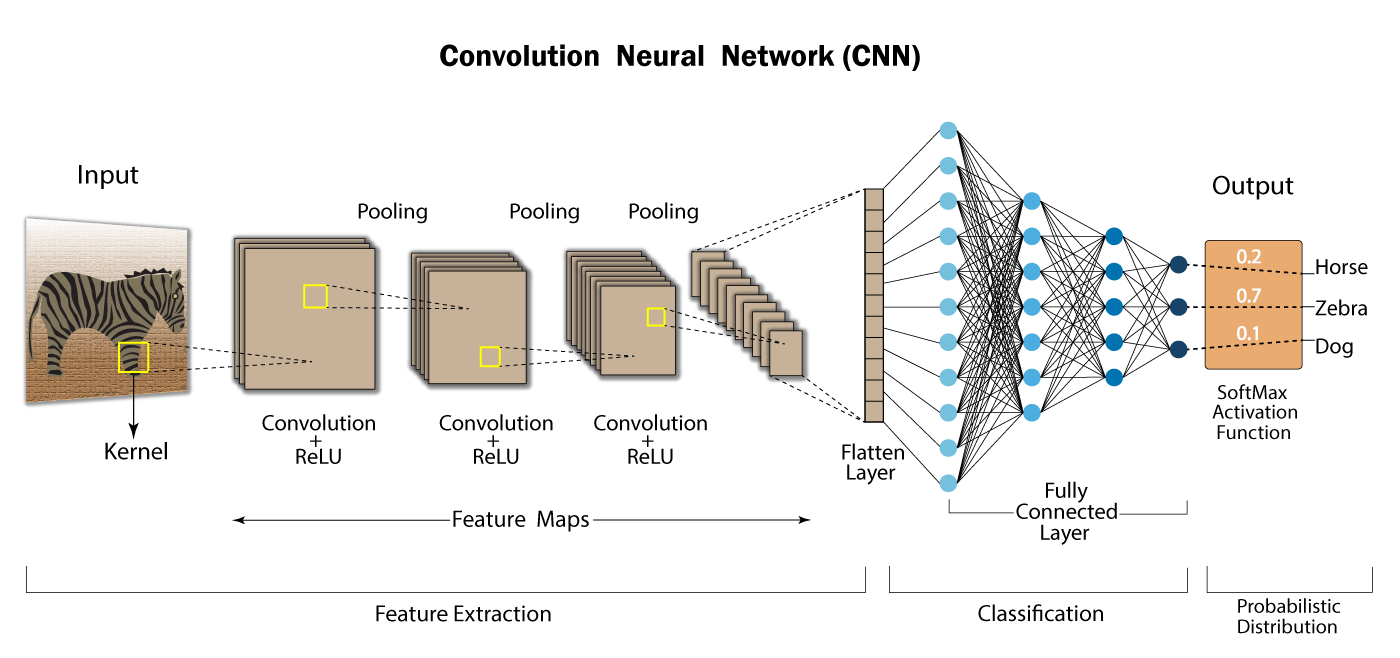
\includegraphics[scale=0.33]{figures/cnn_banner.png}
  Fonte: \href{https://developersbreach.com/convolution-neural-network-deep-learning/}{Developers Breach}. Acesso 13 de mai. 2021.
\end{figure}


\subsubsubsection{\textit{Memória de Longo e Curto Prazo} (\textit{Long Short-Term Memory} ou LSTM)}

\par
As LSTMs são redes neurais recorrentes, e foram introduzidas por Hochreiter \& Schmidhuber (1997). Possuem uma vasta aplicação em inúmeras áreas e são extensamente utilizadas no mercado financeiro \cite{castelao}. A técnica LSTM também apresenta resultados eficientes nas áreas de reconhecimento de voz, reconhecimento de dígitos escritos à mão, entre outros \cite{GoodBengCour16}.

%---------------FIGURE
\begin{figure}[hbt]
\centering
\caption{Representação de uma unidade LSTM, com componentes estruturais e operações matemáticas.}
  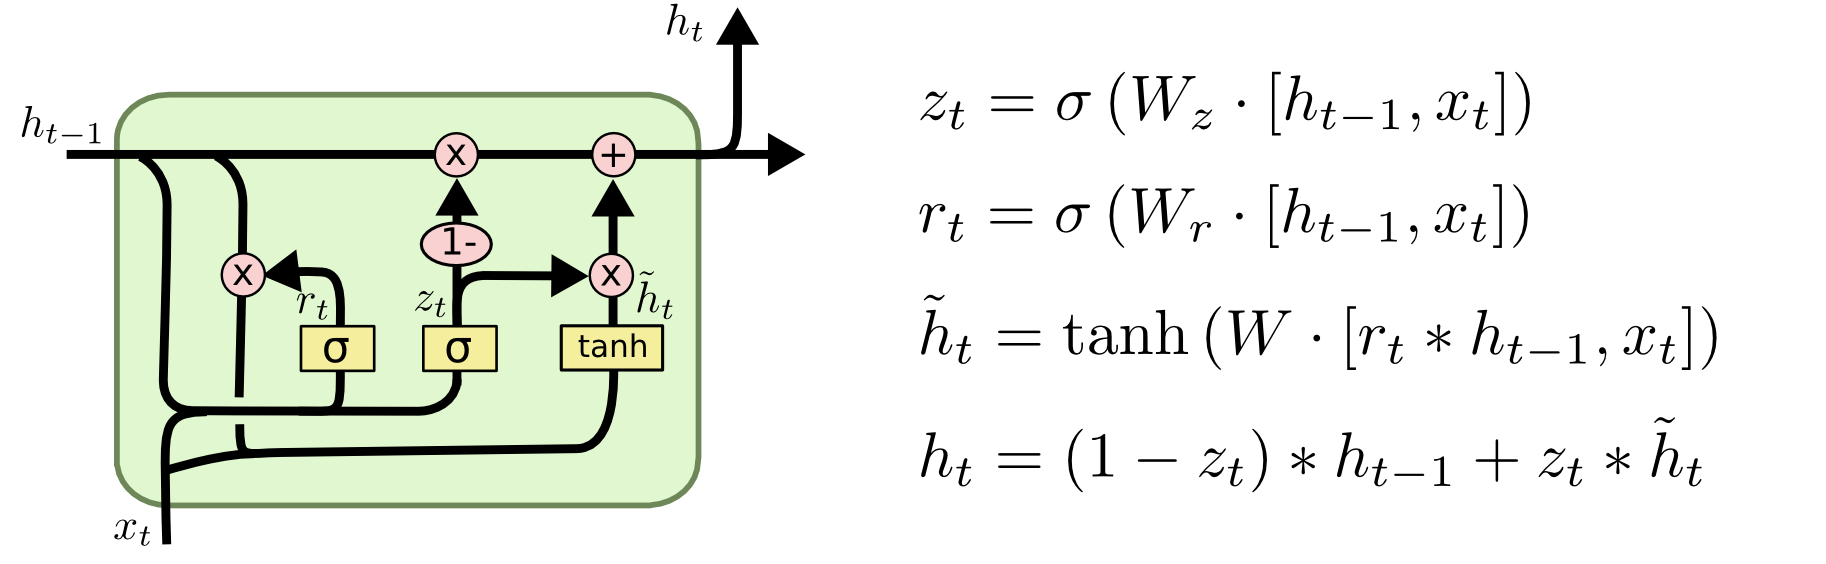
\includegraphics[scale=0.56]{figures/lstm.png} \\
  Fonte: \href{http://colah.github.io/posts/2015-08-Understanding-LSTMs/}{Colah's Blog}. Acesso 13 de mai. 2021.
\end{figure}

% Capítulo 4 - Materiais e Método
\chapter{Materiais e Método}


%---------------------------------------------------------------------------SUB MATERIAIS
\subsection{\textbf{Materiais}}

\par
Em relação ao ambiente de execução, foram utilizados dois ambientes: o primeiro foi o Google Colab para a análise dos resultados e exploração dos dados históricos das ações, utilizando Python em sua versão 3.7.10 (x64); o segundo foi o PyCharm utilizando Python 3.7.0 (x64), destinado para o processamento dos modelos e geração dos resultados. Para possibilitar a implementação das técnicas de Deep Learning (CNN e LSTM) e do modelo Autorregressivo utilizados, bem como a aplicação dos algoritmos e transformações dos dados, algumas bibliotecas da linguagem Python compuseram uma referência base para sua concretização, e estão contidas na tabela abaixo:


%---------------TABLE
\begin{table}[htp]
    \footnotesize
        \caption{Bibliotecas utilizadas, suas respectivas versões e propósitos.}
        \begin{tabular}{cccll}
            \cline{1-3}
            \textbf{Bibliotecas} & \textbf{Versão} & \textbf{Descrição} &  &  \\ \cline{1-3}
            {\fontfamily{cmtt}\selectfont numpy} & 1.19.5 & funções   matemáticas e transformações de matrizes &  &  \\
            {\fontfamily{cmtt}\selectfont matplotlib} & 3.2.2 & plotagem   de gráficos &  &  \\
            {\fontfamily{cmtt}\selectfont pandas\_datareader} & 0.9.0 & carregamento   dos dados históricos, API do yahoo &  &  \\
            {\fontfamily{cmtt}\selectfont pandas} & 1.1.5 & carregamento   e transformações de dados &  &  \\
            {\fontfamily{cmtt}\selectfont sklearn} & 0.22.2.post1 & métricas   para avaliação e pré-processamento dos dados &  &  \\
            {\fontfamily{cmtt}\selectfont datetime} & \textit{defaut} & transformações   de datas &  &  \\
            {\fontfamily{cmtt}\selectfont statsmodels} & 0.10.2 & modelo   Autorregressivo &  &  \\
            {\fontfamily{cmtt}\selectfont keras} & 2.4.3 & modelos CNN e LSTM &  &  \\ \cline{1-3}
        \end{tabular}
        \label{tab:tabela1}
    \center{Fonte: Autor do relatório.}
\end{table}


\par{
Com relação ao hardware referente ao processamento e execução dos algoritmos, o ambiente utilizado foi:}


%---------------TABLE
\begin{table}[htp]
\footnotesize
\centering
\caption{Características de hardware do ambiente de processamento utilizado.}
\begin{tabular}{llcll}
\cline{1-2}
\multicolumn{1}{c|}{CPU} & Intel(R) Core(TM) i7-7700HQ CPU @ 2.80GHz & \textbf{} &  &  \\
\multicolumn{1}{c|}{Memória RAM} & 16GB &  &  &  \\
\multicolumn{1}{c|}{GPU} & NVIDIA GeForce GTX 1050 Ti &  &  &  \\
\multicolumn{1}{c|}{Sistema Operacional (SO)} & Microsoft Windows 10 Pro (x64) &  &  &  \\
\multicolumn{1}{c|}{Versão do SO} & 10.0.19042 N/A compilação 19042 &  &  &  \\
\multicolumn{1}{c|}{Modelo do sistema} & Nitro AN515-51 &  &  &  \\
\multicolumn{1}{c|}{Tipo de sistema} & x64-based PC &  &  &  \\ \cline{1-2}
\end{tabular}
\center{Fonte: Autor do relatório.}
\end{table}


%---------------------------------------------------------------------------SUB MÉTODO
\subsection{\textbf{Método}}

\par
O método empregado visa a mensuração e a comparação entre modelos relacionadas à Séries Temporais Financeiras, tratando-se de um método quantitativo, considerando que utiliza de uma abordagem estatística no que tange à comparação das técnicas existentes, a fim de estabelecer hipóteses de situações potenciais de uso destas, bem como identificá-las mediante análise \cite{wainer}.

\par
As redes neurais testadas (CNN e LSTM) foram treinadas com os preços de fechamento de cada dia dos períodos escolhidos, e então foi testada para um ano posterior ao ano final de treino. As saídas foram numéricas, e então comparadas com os fechamentos reais do ano em questão que foi realizado o teste. Para as saídas geradas, também, foi submetido um algoritmo que compara o preço atual previsto com o preço previsto do dia seguinte, e então classifica-o em “subida” ou “descida”; tais classificações foram comparadas aos movimentos reais obtidos nos fechamentos reais de cada dia, no caso se o preço do dia seguinte foi maior que o atual (subida), ou então foi menor que o atual (descida).

\par
As técnicas de redes neurais CNN e LSTM foram testadas em diferentes períodos, e o experimento foi repetido 10 vezes para cada período devido aos processos estocásticos que ocorrem internamente no funcionamento das redes neurais. Os resultados obtidos foram comparados entre as técnicas, bem como os resultados dos processos de simulação de operação na bolsa de valores.


%---------------------------------------------------------------------------subsub Características dos Dados
\subsubsection{Características dos Dados}


%---------------FIGURE
\begin{figure}[hbt]
\centering
\caption{Dados históricos da ação PETR4.SA (Petrobrás), no ano de 2020.}
  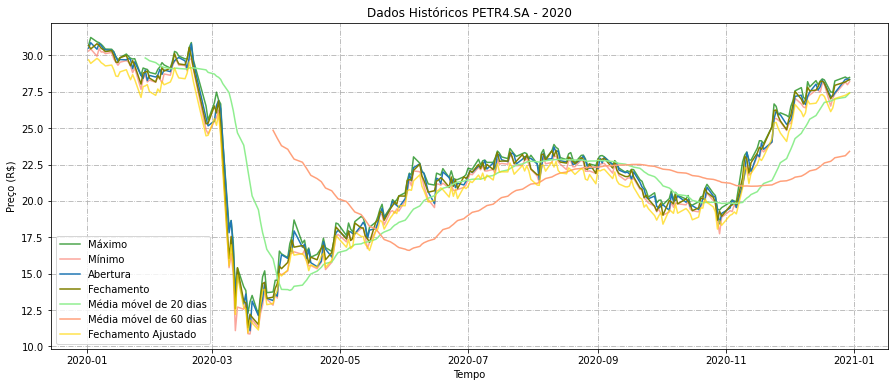
\includegraphics[scale=0.52]{figures/img2.png}
  Fonte: \href{https://finance.yahoo.com/}{Yahoo Finance}. Acesso em 14 mai. 2021.
\end{figure}


%---------------FIGURE
\begin{figure}[H]
\centering
\caption{(a) Altas e baixas; (b) Aberturas e fechamentos; ações PETR4.SA, ano de 2020.}
  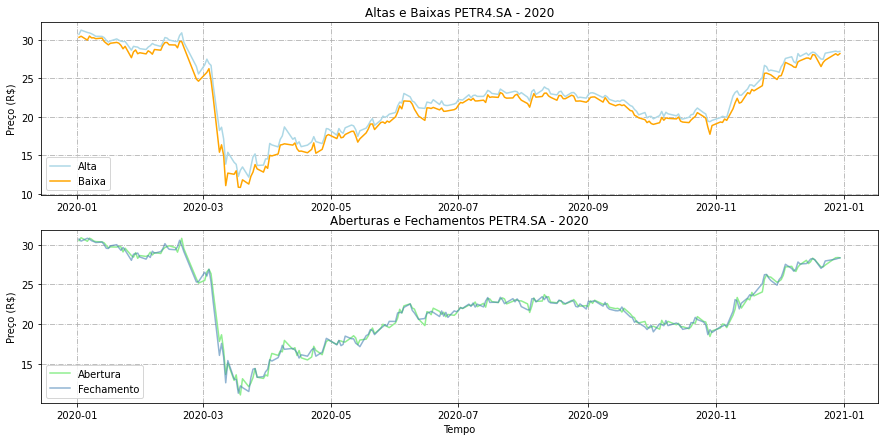
\includegraphics[scale=0.52]{figures/img3.png}
  Fonte: \href{https://finance.yahoo.com/}{Yahoo Finance}. Acesso em 14 mai. 2021.
\end{figure}


%---------------FIGURE
\begin{figure}[H]
\centering
\caption{Dados históricos das cotações em formato de \textit{candlestick}; ações PETR4.SA, ano de 2020.}
  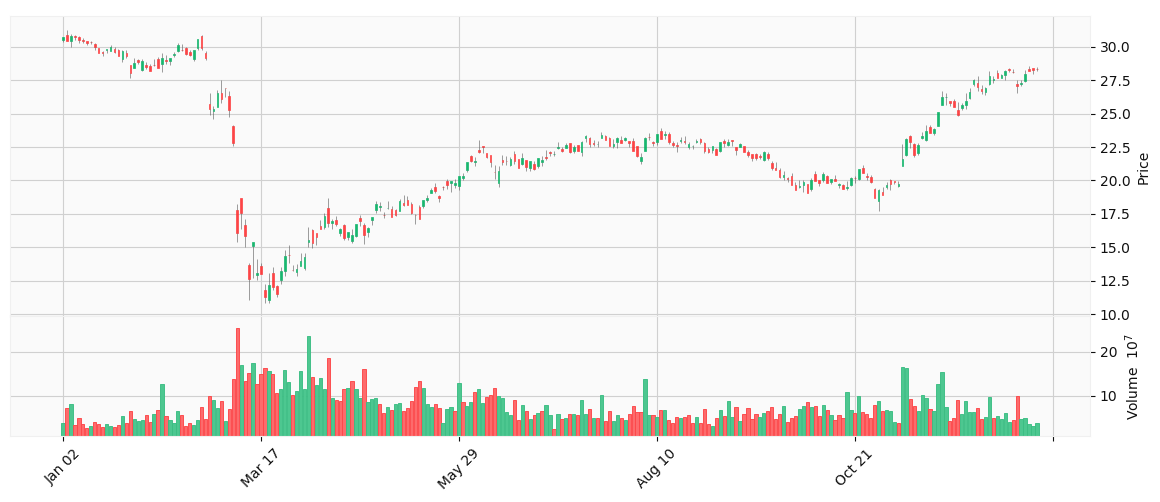
\includegraphics[scale=0.55]{figures/img4.png}
  Fonte: \href{https://finance.yahoo.com/}{Yahoo Finance}. Acesso em 14 mai. 2021.
\end{figure}


%---------------FIGURE
\begin{figure}[H]
\centering
\caption{Retornos diários; ações PETR4.SA, 2020.}
  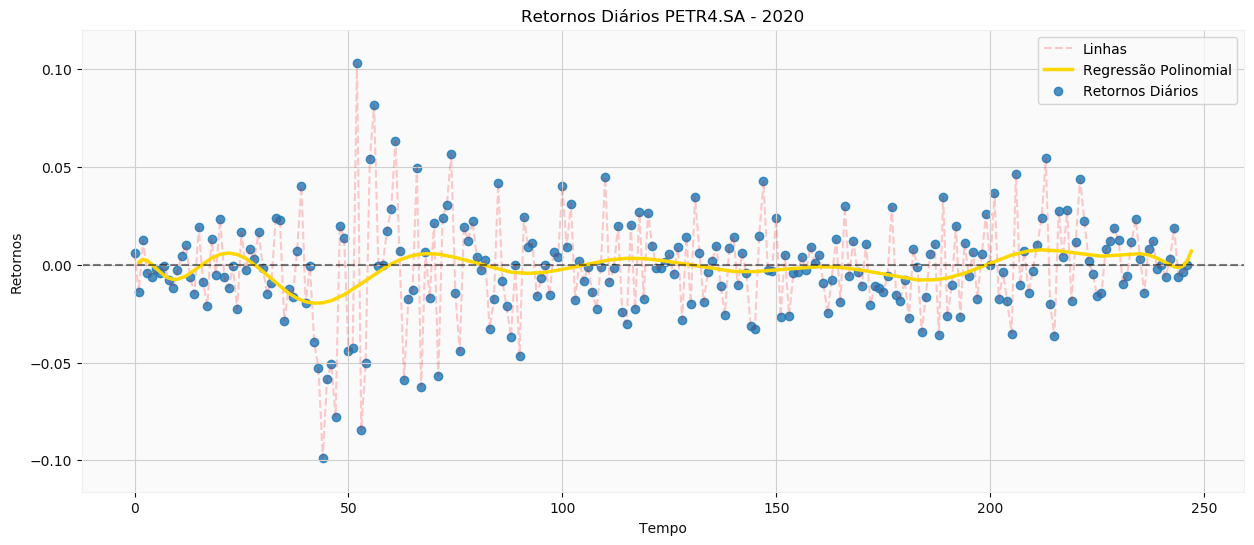
\includegraphics[scale=0.52]{figures/img5.png}
  Fonte: O autor do relatório.
\end{figure}


%---------------TABLE
\begin{table}[H]
\footnotesize
\centering
\caption{Estatísticas sobre os dados históricos da ação PETR4.SA, para o ano de 2020.}
\begin{tabular}{lccll}
\cline{1-3}
\multicolumn{1}{c}{\textbf{Métricas}} & \textbf{2019} & \textbf{2020} &  &  \\ \cline{1-3}
\textit{Contagem} & 247 & 247 &  &  \\
\textit{Média} & 27.248988 & 22.287895 &  &  \\
\textit{Std} & 1.655566 & 4.605092 &  &  \\
\textit{Min} & 23.910000 & 11.290000 &  &  \\
\textit{25\%} & 26.065000 & 19.639999 &  &  \\
\textit{50\%} & 27.129999 & 22.120001 &  &  \\
\textit{75\%} & 28.220000 & 25.710000 &  &  \\
\textit{Max} & \multicolumn{1}{l}{30.969999} & \multicolumn{1}{l}{30.809999} &  &  \\ \cline{1-3}
\end{tabular}
\center{Fonte: Autor do relatório.}
\end{table}


%---------------------------------------------------------------------------subsub Treino e teste do CNN e LSTM
\subsubsection{Treino e teste do CNN e LSTM}

\par
O treino dos modelos, individualmente, foi dividido em diferentes períodos para uma maior variabilidade nos resultados, objetivando submeter o modelo a diferentes situações e registrar seu desempenho. Cada período corresponde a um experimento realizado, seguido da operação simulada na bolsa e a coleta das métricas. Os períodos considerados para treino, teste e simulação de operação de trading, para o CNN e o LSTM foram:


%---------------TABLE
\begin{table}[htp]
\footnotesize
\centering
\caption{Períodos de treino e teste.}
\begin{tabular}{lllll}
\cline{1-4}
\multicolumn{1}{c}{\textbf{Período}} & \multicolumn{1}{c}{\textbf{Treino}} & \multicolumn{1}{c}{\textbf{Teste}} & \multicolumn{1}{c}{\textbf{Resumo}} &  \\ \cline{1-4}
\multicolumn{1}{c}{Período   1} & \multicolumn{1}{c}{01/01/2010    à  31/12/2018} & \multicolumn{1}{c}{01/01/2019    à  31/12/2019} & \multicolumn{1}{c}{2010-2018:   \textit{Treino};  2019: \textit{Teste}} &  \\
\multicolumn{1}{c}{Período   2} & \multicolumn{1}{c}{01/01/2010    à  31/12/2019} & \multicolumn{1}{c}{01/01/2020    à  31/12/2020} & \multicolumn{1}{c}{2010-2019:   \textit{Treino};  2020: \textit{Teste}} &  \\
\multicolumn{1}{c}{Período   3} & \multicolumn{1}{c}{01/01/2010    à  31/12/2018} & \multicolumn{1}{c}{01/01/2020    à  31/12/2020} & \multicolumn{1}{c}{2010-2018: \textit{Treino};  2020:   \textit{Teste}} &  \\ \cline{1-4}
\end{tabular}
\center{Fonte: Autor do relatório.}
\end{table}


%---------------TABLE
\begin{table}[htp]
\footnotesize
\centering
\caption{Períodos de simulação de operação (\textit{trading}).}
\begin{tabular}{lllll}
\cline{1-3}
\multicolumn{1}{c}{\textbf{Período}} & \multicolumn{1}{c}{\textbf{Início   trading}} & \multicolumn{1}{c}{\textbf{Fim   trading}} &  &  \\ \cline{1-3}
\multicolumn{1}{c}{Período   1} & \multicolumn{1}{c}{01/01/2019} & \multicolumn{1}{c}{31/12/2019} &  &  \\
\multicolumn{1}{c}{Período   2} & \multicolumn{1}{c}{01/01/2020} & \multicolumn{1}{c}{31/12/2020} &  &  \\
\multicolumn{1}{c}{Período   3} & \multicolumn{1}{c}{01/01/2020} & \multicolumn{1}{c}{31/12/2020} &  &  \\ \cline{1-3}
\end{tabular}
\center{Fonte: Autor do relatório.}
\end{table}


%---------------TABLE
\begin{table}[H]
\footnotesize
\centering
\caption{Divisão percentual, dos períodos de treino, teste e operação, em percentuais (os intervalos de teste e trading são os mesmos para cada período).}
\begin{tabular}{lllll}
\cline{1-4}
\multicolumn{1}{c}{\textbf{Período}} & \multicolumn{1}{c}{\textbf{Treino}} & \multicolumn{1}{c}{\textbf{Teste}} & \multicolumn{1}{c}{\textbf{Trading}} &  \\ \cline{1-4}
\multicolumn{1}{c}{Período   1} & \multicolumn{1}{c}{89\%} & \multicolumn{1}{c}{11\%} & \multicolumn{1}{c}{11\%} &  \\
\multicolumn{1}{c}{Período   2} & \multicolumn{1}{c}{90\%} & \multicolumn{1}{c}{10\%} & \multicolumn{1}{c}{10\%} &  \\
\multicolumn{1}{c}{Período   3} & \multicolumn{1}{c}{89\%} & \multicolumn{1}{c}{11\%} & \multicolumn{1}{c}{11\%} &  \\ \cline{1-4}
\end{tabular}
\center{Fonte: Autor do relatório.}
\end{table}


%---------------------------------------------------------------------------subsub
\subsubsection{Parâmetros dos modelos utilizados}

\begin{itemize}
\item{CNN}
\end{itemize}
 
\par
A rede foi treinada com o atributo “\textit{close}” de cada dia durante o período de treino, que corresponde ao preço de fechamento da ação naquele dia. As saídas geradas foram números que buscaram prever a ação do dia seguinte. Um algoritmo recebeu tais valores numéricos previstos e retornou as classificações de “alta” ou “baixa” para o dia de hoje, comparando com o preço de amanhã. Abaixo, segue o trecho do código com os parâmetros utilizados nos testes com o CNN:


%---------------CODE
\begin{figure}[hbt]
\caption{Parâmetros utilizados para o treino da rede CNN.}
\lstinputlisting[language=Python]{codes/params1.py}
\center{Fonte: Autor do relatório.}
\end{figure}

\begin{itemize}
\item{LSTM}
\end{itemize}

\par
De maneira semelhante à rede CNN, a rede LSTM foi utilizada para o treino com os preços de fechamentos das ações. A figura abaixo é um trecho de código com a declaração do modelo e os parâmetros utilizados nos testes:


%---------------CODE
\begin{figure}[H]
\caption{Parâmetros utilizados nos testes com a rede LSTM.}
\lstinputlisting[language=Python]{codes/params2.py}
\center{Fonte: Autor do relatório.}
\end{figure}


\begin{itemize}
\item{Modelo \textit{Naive}}
\end{itemize}

\par
O Modelo \textit{Naive} (Modelo “Ingênuo”, do inglês “\textit{naive}”) se refere a um modelo utilizado como base de comparação para as redes neurais. A palavra “ingênuo” se refere à simplicidade do modelo: todas as “previsões” de um período \textit{p} são obtidas por meio do valor do período $p-1$. Dessa forma, todas as previsões são “projeções” dos dados para o futuro; em linhas gerais, representa a confiança de que os dados obtidos no passado se repetirão no presente (daí o termo “ingênuo”).

\begin{itemize}
\item{Modelo Autorregressivo (AR)}
\end{itemize}

\par
Outro modelo utilizado para comparar com os resultados obtidos pelas redes neurais é o modelo Autorregressivo. Este modelo pertence à família de modelos estatísticos tradicionais para a previsão em séries temporais; por ser robusto, foi utilizado neste trabalho para trazer uma base comparativa.

\par
Para o modelo Autorregressivo, foram utilizados 60 dias anteriores ao período de teste e operação para o treino. Por exemplo, para o teste e treino no ano de 2019, o modelo utilizou 60 dias do final de 2018 para treiná-lo. O parâmetro \textit{endog} do modelo foi o conjunto de preços de fechamento, e o \textit{maxlag} foi 60.

%---------------------------------------------------------------------------SUB
\subsection{\textbf{Algoritmos de Trading}}

São os algoritmos que realizam a simulação da operação de trading na bolsa de valores, cada um com uma regra específica associada à tomada de decisão.


%---------------------------------------------------------------------------subsub
\subsubsection{Algoritmo \textit{Classifications Trading} (CT)}

\par
Algoritmo de Trading que utiliza as classificações de “alta” ou “baixa” para o dia seguinte (em relação ao preço de fechamento) para tomar decisões a respeito da compra ou venda de ações \cite{ritzmann}. Resumidamente, o algoritmo irá se basear na previsão do dia de hoje, comparando se o movimento previsto de hoje em relação a amanhã será de baixa ou alta. Por exemplo, o modelo CNN previu o valor R\$ 26,88 para o fechamento de amanhã, e o fechamento de hoje é de R\$ 24,90, logo será classificado como “alta” para hoje, pois amanhã o preço de fechamento subirá, logo o algoritmo fará uma compra.


%---------------FIGURE
\begin{figure}[hbt]
\centering
\caption{\label{figure:figura1}: Fluxograma do algoritmo “\text{\textit{Classifications Trading}}”.}
  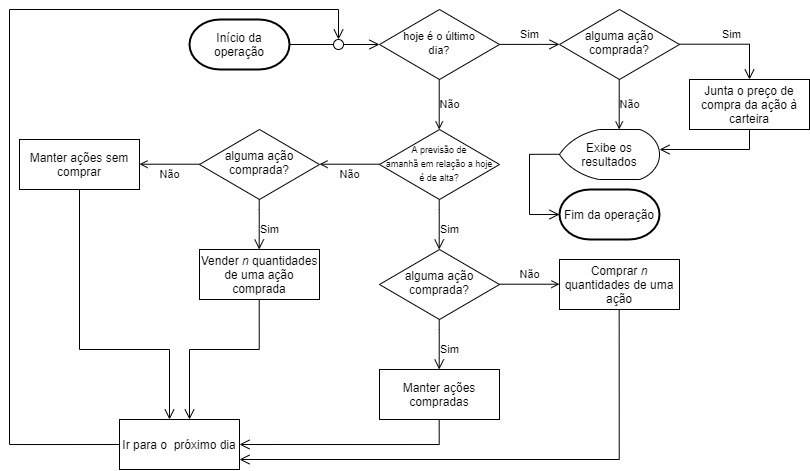
\includegraphics[scale=0.55]{figures/Classifications_Trading.png}
  Fonte: O autor do relatório.
\end{figure}


%---------------PSEUDOCODE
\begin{algorithm}[H]
\caption{Pseudocódigo do algoritmo \textit{classifications\_trading}(\textit{c}, $ \vec{p_c} $, $ \vec{p_p} $)}
\scriptsize
\textbf{Entrada}: Carteira inicial \textit{c}; preços reais de fechamento $ \vec{p_c} $; preços previstos de fechamento $ \vec{p_p} $
\begin{algorithmic}[1]
\footnotesize
\Function{ClassificationsTrading}{\textit{c}, $ \vec{p_c} $, $ \vec{p_p} $}
    \State $ultima\_compra\gets 0$
    \State $acao\_comprada\gets falso$
        \For{$dia$}{$hoje$}{$ultimo\_dia$}
            \If {$hoje == ultimo\_dia$}
                \State $c \gets c + ultima\_compra$
            \Else
                \If {$\vec{p_p}[dia] == subida $}
                    \If {$acao\_comprada == verdadeiro $}
                        \State $continuar$
                    \Else
                        \State $comprar\_acao(n\_acoes)$
                        \State $acao\_comprada = verdadeiro$
                    \EndIf
                \Else
                    \If {$acao\_comprada == verdadeiro $}
                        \State $vender\_acao(n\_acoes)$
                        \State $acao\_comprada = falso$
                    \Else
                        \State $continuar$
                    \EndIf
                \EndIf
            \EndIf
        \EndFor
\EndFunction
\end{algorithmic}
\end{algorithm}


%---------------------------------------------------------------------------subsub
\subsubsection{Algoritmo \textit{Naive Trading} (NT)}


\par
Algoritmo de Trading que utiliza uma técnica ingênua para tomada de decisão. Se o preço de fechamento de ontem for menor que o preço de fechamento de antes de ontem, infere-se que o mercado está em queda, portanto as ações serão vendidas. Caso contrário, ou seja, o preço de ontem é maior que o de antes de ontem, então compramos ações. A ideia desse algoritmo é ter uma base de comparação próxima do real, para os casos de compra e venda sem técnicas sofisticadas e afins, de maneira a averiguar o desempenho de tal técnica em relação às previsões provenientes das redes neurais.


%---------------PSEUDOCODE
\begin{algorithm}[H]
\caption{Pseudocódigo do algoritmo \textit{naive\_trading}(\textit{c}, $ \vec{p_c} $)}
\scriptsize
\textbf{Entrada}: Carteira inicial \textit{c}; preços reais de fechamento $ \vec{p_c} $;
\begin{algorithmic}[1]
\footnotesize
\Function{NaiveTrading}{\textit{c}, $ \vec{p_c} $}
    \State $ultima\_compra\gets 0$
    \State $acao\_comprada\gets falso$
        \For{$dia$}{$hoje$}{$ultimo\_dia$}
            \If {$hoje == ultimo\_dia$}
                \State $c \gets c + ultima\_compra$
            \Else
                \If {$\vec{p_c}[dia-1] > \vec{p_c}[dia-2]$}
                    \If {$acao\_comprada == verdadeiro $}
                        \State $continuar$
                    \Else
                        \State $comprar\_acao(n\_acoes)$
                        \State $acao\_comprada = verdadeiro$
                    \EndIf
                \Else
                    \If {$acao\_comprada == verdadeiro $}
                        \State $vender\_acao(n\_acoes)$
                        \State $acao\_comprada = falso$
                    \Else
                        \State $continuar$
                    \EndIf
                \EndIf
            \EndIf
        \EndFor
\EndFunction
\end{algorithmic}
\end{algorithm}


%---------------------------------------------------------------------------subsub
\subsubsection{Algoritmo \textit{Real Movements Trading} (RMT)}


\par
O algoritmo “\textit{Real Movements Trading}” é, na realidade, o mesmo algoritmo de “Classifications Trading”, com a única diferença que este utiliza os movimentos reais do período de operação, portanto é um algoritmo com 100\% de precisão em relação às operações com lucro. A ideia desse algoritmo é ter uma base de comparação utópica, para um caso perfeito onde saberíamos todos os movimentos reais da bolsa de valores antes mesmo de acontecerem. Por exemplo, o preço de fechamento de amanhã será maior que o de hoje, então o movimento é classificado como “alta”, então o algoritmo efetua a compra de ações para aproveitar o aumento de preço em detrimento de uma compra com valor inferior ao de amanhã; o algoritmo só fará a venda das ações quando o movimento for de “descida”, então venderá todas as ações antes de obter prejuízo.


%---------------------------------------------------------------------------SUB
\subsection{\textbf{Métricas de avaliação utilizadas}}


\par
Os testes com os modelos e as operações foram submetidos à métricas específicas para cada caso. Ao final, foram extraídas as médias e desvio-padrões dos resultados de cada métrica. 


%---------------------------------------------------------------------------subsub
\subsubsection{Métricas de Teste}


\par
As métricas utilizadas para avaliar o desempenho dos modelos em teste, logo após serem treinados e testados durante um ano. As saídas numéricas se referem ao preço de fechamento “previsto” pelo modelo. As saídas categóricas se referem as classificações geradas ao compararem os preços “previstos” para rotulá-las em “alta” ou “baixa”.


%---------------------------------------------------------------------------subsubsub
\subsubsubsection{\textit{Métricas para as Saídas numéricas}}


\begin{itemize}
\item{Coeficiente de determinação (\textit{R squared} ou R2)}
\end{itemize}

É uma medida de ajuste de um modelo linear generalizado, cuja equação é:

\begin{equation}
{\displaystyle SQ_{\text{tot}}=\sum _{i=1}^{n}(y_{i}-{\bar {y}})^{2}}
\end{equation}

Onde \textit{n} é o número de observações, $\mathrm{y_i}$ é o valor observado e \textit{y} é a média das observações.


\begin{itemize}
\item{Erro Quadrático Médio (\textit{Mean Squared Error} ou MSE)}
\end{itemize}

É a média da diferença entre o valor real e previsto, cujo método é:

\begin{equation}
    {\displaystyle EQM({\hat {\theta }})={\frac {1}{N}}\sum _{i=1}^{N}({\hat {\theta _{i}}}-\theta _{i})^{2}}
\end{equation}

Onde $\mathrm{\theta}$ é o valor estimado, $\mathrm{\theta_{i}}$ o valor previsto e \textit{N} o número de observações.


%---------------------------------------------------------------------------subsubsub
\subsubsubsection{\textit{Métricas para as saídas categóricas}}


\begin{itemize}
\item{Medida F (\textit{F1-Score}) \par Medida que utiliza \textit{accuracy}, \textit{precision} e \textit{recall} para gerar um score, cujo método é:}
\end{itemize}


\begin{equation}
F1 = 2 \times \frac{precision \times recall}{precison + recall}
\end{equation}

\begin{itemize}
\item{Acurácia (\textit{Accuracy}) \par Porcentagem de previsões corretas em relação ao total de previsões, cujo método é:}
\end{itemize}


\begin{equation}
accuracy = \frac{TP + TN}{TP + TN + FP + FN}
\end{equation}

\begin{itemize}
\item{Precisão (\textit{Precision}) \par Porcentagem de dados positivos entre todos os classificados como positivos, cujo método é:}
\end{itemize}


\begin{equation}
precision = \frac{TP}{TP+FP}
\end{equation}

\begin{itemize}
\item{Revocação (\textit{Recall}) \par Indica o quão bem o modelo prevê positivos em relação ao total de positivos, cujo método é:}
\end{itemize}


\begin{equation}
recall = \frac{TP}{TP + FN}
\end{equation}


%---------------------------------------------------------------------------subsub
\subsubsection{Métricas para o período de \textit{trading}}

\begin{itemize}
\item{\textit{Carteira final} (CF) \par
Valor da carteira, em R\$, no período final após completar a operação de trading.}
\end{itemize}


\begin{itemize}
\item{\textit{Diferença das carteiras} (DC) \par
Diferença, em R\$, entre a carteira inicial (R\$ 100.000,00) e a carteira final da operação.}
\end{itemize}

\begin{itemize}
\item{\textit{Razão entre as carteiras} (RC) \par
Razão entre a carteira final e a carteira inicial.}
\end{itemize}

\begin{itemize}
\item{\textit{Qtd. De Operações com lucro} (QOL) \par
Dentre as operações realizadas (1 operação é o ato de compra e venda), é o número das que tiveram lucro.}
\end{itemize}


\begin{itemize}
\item{\textit{Qtd. De Operações com perda} (QOP) \par
Dentre as operações realizadas, é o número das que tiveram prejuízo.}
\end{itemize}


\begin{itemize}
\item{\textit{Acurácia de operações com lucro} (AOL) \par
Razão entre as operações com lucro e o total de operações realizadas.}
\end{itemize}


\begin{itemize}
\item{\textit{Ganho médio por operações com lucro, em R\$} (GMO) \par
Dentre as operações com lucro, é a média entre o valor lucrado por operação.}
\end{itemize}


%---------------------------------------------------------------------------SUB
\subsection{\textbf{Ordem dos experimentos realizados}}

\par
Os modelos utilizados, juntamente com os algoritmos de trading e os períodos de treino e operação, seguiram a tabela abaixo, que descreve os experimentos realizados:


%---------------TABLE
\begin{table}[htp]
\footnotesize
\centering
\caption{Algoritmo de \textit{trading} escolhido para cada técnica utilizada para realizar previsões, com o respectivo número de ações negociadas em cada operação, e os períodos diferentes para teste e operação.}
\begin{tabular}{ccccc}
\hline
\textbf{Técnica} & \textbf{Algoritmo   Trading} & \textbf{QAC} & \textbf{Período   Trading} & \textbf{Repetições} \\ \hline
CNN & Classificações & 1500 & Período   1, 2 e 3 & 10   vezes p/ cada período \\
LSTM & Classificações & 1500 & Período   1, 2 e 3 & 10   vezes p/ cada período \\
Modelo   Naive & Classificações & 1500 & 2019   e 2020 & 1   vez p/ cada período \\
Autorregressivo & Classificações & 1500 & 2019   e 2020 & 1   vez p/ cada período \\
Modelo   Naive & Classificações & 1500 & 2019   e 2020 & 1   vez p/ cada período \\
Sem   modelo & Naive   Trading & 1500 & 2019   e 2020 & 1   vez p/ cada período \\
Sem   modelo & Movimentos   Reais & 1500 & 2019   e 2020 & 1 vez p/ cada período \\ \hline
\end{tabular}
\center{Fonte: Autor do relatório.}
\end{table}


%---------------FIGURE
\begin{figure}[hbt]
\centering
\caption{\label{figure:figura1}Fluxograma adaptado dos experimentos realizados, com diagrama incluindo treino e teste de diferentes modelos em diferentes períodos, bem como a operação de \textit{trading} com diferentes algoritmos.}
  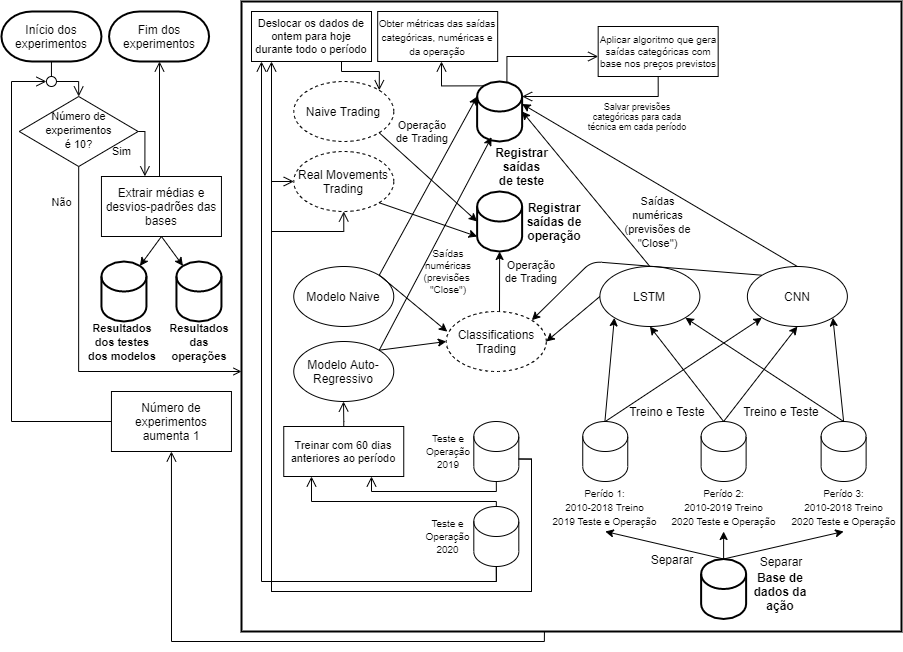
\includegraphics[scale=0.52]{figures/img17.png}
  Fonte: O autor do relatório.
\end{figure}

% Capítulo 5 - Resultados
\chapter{Resultados}

\par
Após realizar os experimentos para as ações PETR4.SA (Petrobrás), os modelos foram treinados, testados e avaliados em diferentes períodos, bem como suas previsões utilizadas em simulações de operações de trading. Os resultados dos 10 experimentos de cada período do CNN e LSTM foram submetidos à média e ao desvio padrão, e os demais testados para o ano de 2019 e 2020, posteriormente submetidos à média e desvio padrão também. Os gráficos de operações de trading abaixo são experimentos retirados dos testes feitos.


%---------------------------------------------------------------------------SUB

\subsection{\textbf{Previsões com CNN e Operações com Classifications Trading}}


%---------------FIGURE
\begin{figure}[hbt]
\centering
\caption{\label{figure:figura1}Previsões do CNN, seguido dos preços de fechamento reais e as operações de compra e venda, para 2020.}
  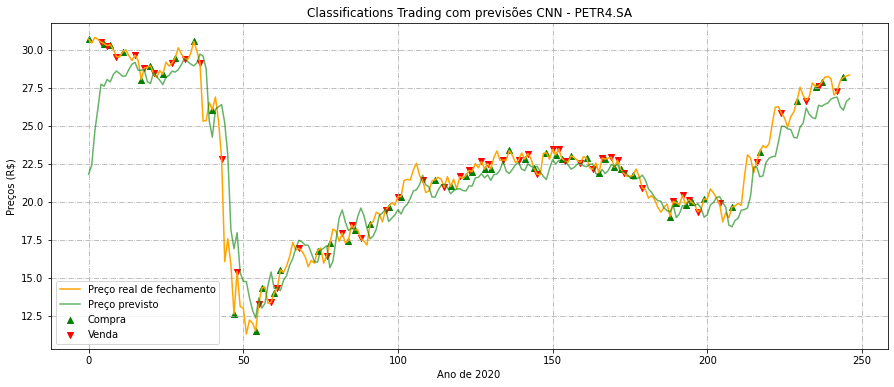
\includegraphics[scale=0.5]{figures/img18.png}
  Fonte: O autor do relatório.
\end{figure}


%---------------------------------------------------------------------------SUB

\subsection{\textbf{Previsões com LSTM e Operações com \textit{Classifications Trading}}}


%---------------FIGURE
\begin{figure}[H]
\centering
\caption{\label{figure:figura1}Previsões do LSTM, seguido dos preços de fechamento reais e as operações de compra e venda, para 2020.}
  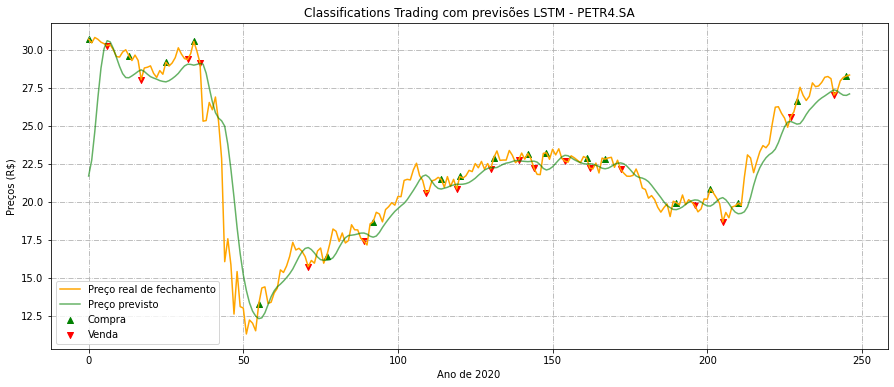
\includegraphics[scale=0.5]{figures/img19.png}
  Fonte: O autor do relatório.
\end{figure}

\subsection{Operações com \textit{Naive Trading}}


%---------------FIGURE
\begin{figure}[hbt]
\centering
\caption{\label{figure:figura1}Operações do algoritmo \textit{Naive Trading}, sem modelo, para o ano de 2020.}
  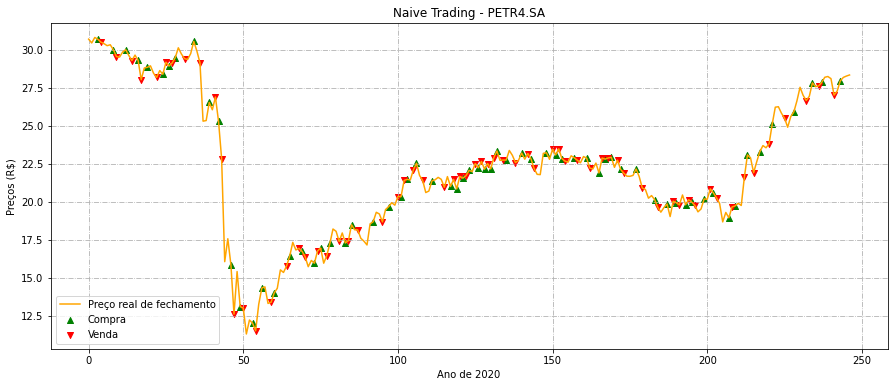
\includegraphics[scale=0.5]{figures/img13.png}
  Fonte: O autor do relatório.
\end{figure}

%---------------------------------------------------------------------------SUB

\subsection{\textbf{Médias dos resultados dos testes com as saídas numéricas}}


%---------------TABLE
\begin{table}[H]
\footnotesize
\centering
\caption{Médias dos resultados de todos os períodos dos testes feitos com cada técnica treinada, utilizando as saídas numéricas geradas pelo algoritmo e comparando os preços de fechamento com os preços reais observados.}
\begin{tabular}{ccccc}
\hline
\textbf{Técnica} & \textbf{Ação} & \textbf{Período} & \textbf{R2} & \textbf{MSE $({R\$})^{2}$} \\ \hline
CNN & PETR4.SA & Todos & 0.825285 & 1.736832 \\
LSTM & PETR4.SA & Todos & 0.923408 & 0.769675 \\
Modelo   Naive & PETR4.SA & Todos & 0.938442 & 0.475895 \\
AR & PETR4.SA & Todos & \textbf{0.955583} & \textbf{0.323019} \\ \hline
\end{tabular}
\center{Fonte: Autor do relatório.}
\end{table}

%---------------------------------------------------------------------------SUB

\subsection{\textbf{Médias dos resultados dos testes com as saídas categóricas}}


%---------------TABLE
\begin{table}[htp]
\footnotesize
\centering
\caption{Médias dos resultados de todos os períodos dos testes feitos com cada técnica, utilizando as classificações geradas pelo algoritmo e comparando os movimentos classificados como “alta” e “baixa” com os movimentos reais.}
\begin{tabular}{ccccccc}
\hline
\textbf{Técnica} & \textbf{Ação} & \textbf{Período} & \textbf{F1-Score} & \textbf{Acurácia} & \textbf{Precisão} & \textbf{Revocação} \\ \hline
CNN & PETR4.SA & Todos & \textbf{0.548317} & 0.527642 & 0.530769 & \textbf{0.567882} \\
LSTM & PETR4.SA & Todos & 0.480198 & 0.469783 & 0.47492 & 0.485627 \\
Modelo   Naive & PETR4.SA & Todos & 0.488195 & 0.477642 & 0.487201 & 0.489198 \\
AR & PETR4.SA & Todos & \textbf{0.595666} & \textbf{0.583006} & \textbf{0.588752} & \textbf{0.60276} \\ \hline
\end{tabular}
\center{Fonte: Autor do relatório.}
\end{table}


%---------------------------------------------------------------------------SUB
\subsection{\textbf{Médias dos resultados das operações}}


%---------------TABLE
\begin{table}[htp]
\scriptsize
\centering
\caption{Médias dos resultados de todos os períodos dos testes feitos com cada técnica combinada a um algoritmo de \textit{trading}.}
\begin{tabular}{cccccccc}
\hline
\textbf{Técnica} & \textbf{Ação} & \textbf{Período} & \textbf{ET} & \textbf{CI   (R\$)} & \textbf{CF   (R\$)} & \textbf{DC   (R\$)} & \textbf{RC} \\ \hline
CNN & PETR4.SA & Todos & Class.   T. & 100000.0 & 111,145.493793 & 11,145.493793 & \textbf{1.1114} \\
LSTM & PETR4.SA & Todos & Class.   T. & 100000.0 & 96,990.799319 & -3,009.200681 & 0.96990 \\
\textit{Modelo   Naive} & PETR4.SA & Todos & Class.   T. & 100000.0 & 80,634.992361 & -19,365.007639 & 0.80635 \\
AR & PETR4.SA & Todos & Class.   T. & 100000.0 & 127,029.992104 & 27,029.992104 & \textbf{1.2703} \\
Não   possui & PETR4.SA & Todos & \textit{Naive   Trading} & 100000.0 & 100,104.996681 & 104.996681 & 1.0010 \\
Não   possui & PETR4.SA & Todos & RMT & 100000.0 & 184,105.011702 & 84,105.011702 & \textbf{1.8410} \\ \hline
\end{tabular}
\center{Fonte: Autor do relatório.}
\end{table}


%---------------TABLE
\begin{table}[htp]
\footnotesize
\centering
\caption{Médias dos resultados de todos os períodos dos testes feitos com cada técnica combinada a um algoritmo de \textit{trading}.}
\begin{tabular}{cccccccc}
\hline
\textbf{Técnica} & \textbf{Ação} & \textbf{Período} & \textbf{ET} & \textbf{QOL} & \textbf{QOP} & \textbf{AOL} & \textbf{GMO   (R\$)} \\ \hline
CNN & PETR4.SA & Todos & Class.   T. & 33.5 & 22.7 & \textbf{0.595812} & 196.77536 \\
LSTM & PETR4.SA & Todos & Class.   T. & 19.5 & 33.0 & 0.372729 & -56.297246 \\
Modelo   \textit{Naive} & PETR4.SA & Todos & Class.   T. & 22.0 & 42.5 & 0.340909 & 18.793181 \\
AR & PETR4.SA & Todos & Class.   T. & 40.5 & 25.5 & \textbf{0.615278} & 408.08322 \\
Não   possui & PETR4.SA & Todos & \textit{Naive   Trading} & 31.5 & 32.0 & 0.496898 & 4.217068 \\
Não   possui & PETR4.SA & Todos & RMT & 64.0 & 0.0 & \textbf{1.0} & 1,311.769415 \\ \hline
\end{tabular}
\center{Fonte: Autor do relatório.}
\end{table}

\par
A figura abaixo compara algumas métricas utilizadas em teste, para os modelos CNN e \textit{Naive}; a última métrica representa a acurácia das operações com lucro (AOP), sendo uma métrica utilizada nas operações de trading de ambos os modelos. Essa comparação evidencia o desempenho da rede CNN diante de uma técnica simples de previsão em séries temporais.


%---------------FIGURE
\begin{figure}[hbt]
\centering
\caption{\label{figure:figura1}Comparação das métricas categóricas entre o CNN e o modelo \textit{Naive}, bem como a acurácia média das operações com lucro (última métrica).}
  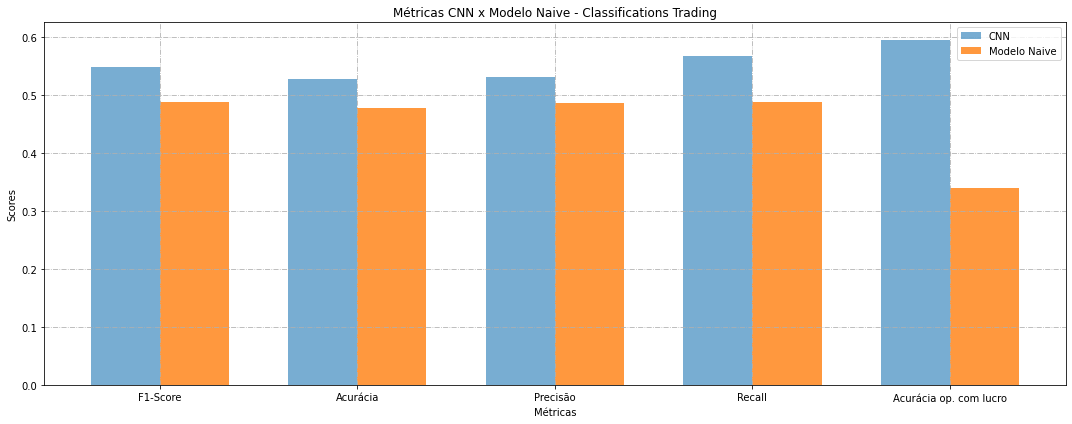
\includegraphics[scale=0.43]{figures/img15.png}
  Fonte: O autor do relatório.
\end{figure}

% Capítulo 6 - Discussão
\chapter{Discussão}

\par
Analisando os resultados das tabelas, podemos observar que os melhores desempenhos foram do modelo Autorregressivo (AR) e a rede neural CNN. Os maiores lucros observados foram de ambos os modelos, com AR fechandouma carteira com +27\% de lucro, e o CNN com a carteira com +11\% de lucro, ambos com o investimento inicial de R\$ 100.000,00.

\begin{figure}[hbt]
\centering
\caption{\label{figure:figura1}Diferentes métricas, na média, para os modelos testados, bem como acurácia das operações com lucro (primeira métrica).}
  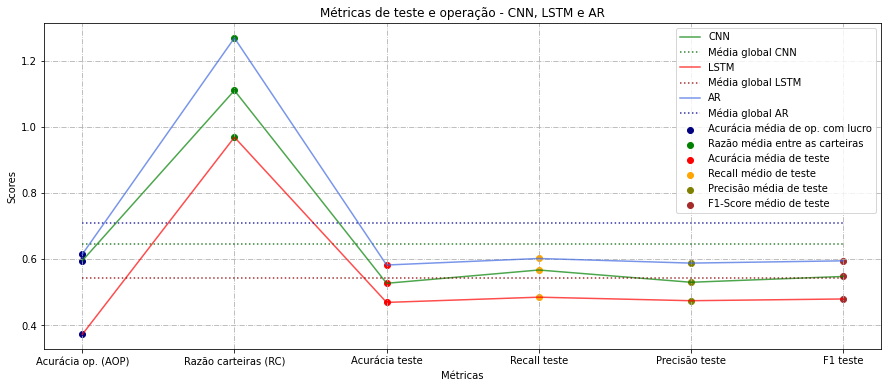
\includegraphics[scale=0.5]{figures/img1.png}
  Fonte: O autor do relatório.
\end{figure}

\par
O AR é um modelo robusto utilizado em previsões em séries temporais, então seu ótimo desempenho foi esperado. Já o modelo LSTM, para os parâmetros aqui testados, não apresentou bons resultados, principalmente se comparado ao CNN. É notável que o LSTM teve as métricas numéricas muito mais precisas que ambos AR e CNN; isso significa que o modelo teve boa capacidade de aproximar o valor previsto do fechamento para o valor real de fechamento, que se ilustra no gráfico de operação do LSTM pela proximidade entre o real e o previsto. Apesar dos valores aproximados, entretanto, as medidas das saídas categóricas ficaram inferiores, tanto no F1-Score quanto na acurácia geral, exemplificando um lucro baixo (ou prejuízo), visto que o lucro é diretamente proporcional aos movimentos classificados corretamente o maior número de vezes possível.

\par
O modelo AR apresentou média global maior que o CNN, mas suas acurácias médias de operações com lucro foram próximas, respectivamente 61\% e 59\%. Apesar das diferenças entre as acurácias no teste dos modelos (AR com 58\% e CNN com 52\%), o lucro final está diretamente relacionado com a porcentagem de operações com lucro, que em ambos os casos estão próximas de 60\%.

\par
A figura abaixo compara as funções densidade de probabilidade entre os valores obtidos nos experimentos de teste e \textit{trading} para o modelo CNN, respectivamente utilizando as métricas de acurácia da previsão dos movimentos e a acurácia de lucro nas operações realizadas.

\begin{figure}[hbt]
\centering
\caption{\label{figure:figura1}Distribuição das acurácias para os experimentos realizados com o CNN, em todos os períodos, bem como as distribuições para as operações que utilizaram as previsões do CNN, para todos os resultados em todos os períodos.}
  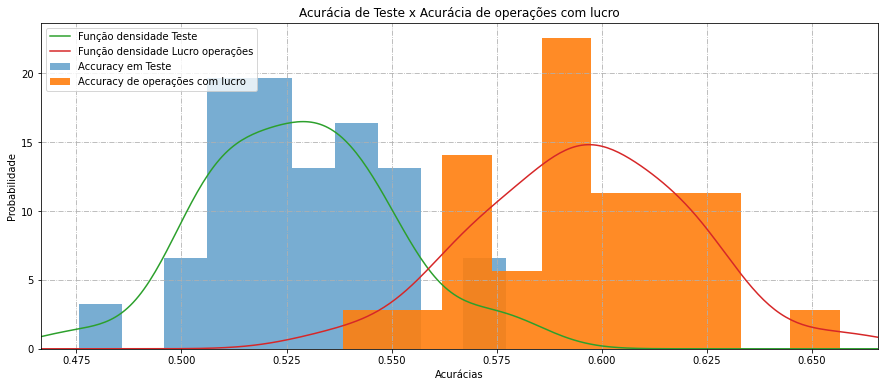
\includegraphics[scale=0.5]{figures/img14.png}
  Fonte: O autor do relatório.
\end{figure}

\par
Podemos notar que, para valores de acurácia em teste que tendem a 0.6, a acurácia de operações com lucro atinge, nessa posição, seu ponto médio. É possível traçar um paralelo entre a acurácia de teste e a acurácia de operação, levantando a hipótese de que existe uma relação diretamente proporcional entre as duas variáveis; esta hipótese também explicaria o porquê do modelo LSTM ter um desempenho ineficiente em operação, contrastando com sua precisão em termos numéricos (R2 e MSE), visto que a proximidade do valor previsto com o real não implica em acertar o movimento das ações; podemos, por exemplo, prever um valor abaixo – ainda que próximo – de uma ação, e equivocadamente classifica-la em “baixa”.

\par
Comparando as métricas de teste e acurácia de acerto em operação do CNN com o Modelo \textit{Naive} (Figura 4.6.1), observamos a maior diferença na acurácia das operações com lucro, que salta de 34\% para 59\% (+73\% de acurácia de acerto). É interessante notar que esse aumento possibilitou uma carteira final aproximadamente +38\% acima do Modelo \textit{Naive}, que na realidade finalizou com uma carteira em 80\% do valor inicial (apresentou prejuízo). Também fica evidente a diferença quando comparamos o ganho médio (em R\$), para as operações com lucro, no qual o CNN apresenta aproximadamente +988\% de lucro.

\par
Comparando o desempenho em operação do CNN com o \textit{Naive} Trading, a acurácia média de operações com lucro foi de +20\% para o CNN, com lucro médio das operações com lucro saltando de R\$ 4,21 para R\$ 192,77. O lucro final das carteiras aqui salta de R\$ 104,99 para R\$ 11.145,49 com o CNN.

\par
O desempenho do CNN frente às técnicas ingênuas, tanto para o modelo \textit{Naive} utilizando Classifications Trading quanto para o \textit{Naive} \textit{Trading} (operando sem modelo), se demonstrou mais eficiente e lucrativo. Entretanto, comparativamente ao modelo AR, seu desempenho em todos os casos foi inferior. Comparativamente, a média das diferenças entre as carteiras finais foi de R\$ 11.145,49 para o CNN, bem como R\$ 27.029,99 para o AR. É interessante notar que as acurácias de lucro por operações são semelhantes (aproximadamente 60\%); para as acurácias máximas observadas durante os experimentos, o CNN teve a AOL atingindo 65\% de operações com lucro, em contrapartida de 63\% para o modelo AR.

\par
Se compararmos o desempenho dos modelos com o algoritmo \textit{Real Movements Trading}, podemos estabelecer um parâmetro de desempenho ótimo, do qual acerta todas as operações, e então avaliar cada técnica individualmente. O RMT fez 64 operações, das quais acertou todas, na média entre os anos 2019 e 2020. Para o CNN, temos 52\% de acerto das operações considerando um desempenho perfeito; no caso do AR temos 63\%; LSTM com 30\%; Modelo \textit{Naive} com 34\%. É notável que o CNN e o AR tiveram desempenhos muito superiores às demais técnicas, e para as métricas, de forma geral, um desempenho próximo de 60\% implica também em 60\% de aproveitamento em relação ao desempenho perfeito.


\par
Considerando como ideal o algoritmo RMT, bem como as métricas do modelo AR todas ótimas, os modelos foram avaliados segundo os critérios abaixo:


%---------------TABLE
\begin{table}[H]
\footnotesize
\centering
\caption{Critérios para avalair os modelos segundo suas métricas.}
\begin{tabular}{ccccc|cll}
\cline{1-6}
0.65 & $\geq$ & \textit{accuracy} & $\geq$ & 0.60 & \textit{ótimo} &  &  \\
0.60 & > & \textit{accuracy} & $\geq$ & 0.55 & \textit{bom} &  &  \\
0.55 & > & \textit{accuracy} & $\geq$ & 0.50 & \textit{razoável} &  &  \\
0.50 & > & \textit{accuracy} & $\geq$ & 0.00 & \textit{ruim} &  &  \\
1.00 & $\geq$ & R2 & $\geq$ & 0.90 & \textit{ótimo} &  &  \\
0.90 & > & R2 & $\geq$ & 0.70 & \textit{bom} &  &  \\
0.70 & > & R2 & $\geq$ & 0.00 & \textit{ruim} &  &  \\
1.00 & $\geq$ & AOL & $\geq$ & 0.55 & \textit{ótimo} &  &  \\
0.55 & > & AOL & $\geq$ & 0.50 & \textit{bom} &  &  \\
0.50 & > & AOL & $\geq$ & 0.00 & \textit{ruim} &  &  \\ \cline{1-6}
\end{tabular}
\center{Fonte: Autor do relatório. Dados das tabelas 8, 9 e 11.}
\end{table}


\par
Para os experimentos realizados neste trabalho, observamos que:

\begin{itemize}
    
    \item{A \textit{rede CNN} apresentou um desempenho \textbf{bom} na classificação dos movimentos}
    \item{A \textit{rede CNN} apresentou um desempenho \textbf{razoável} nas previsões numéricas}
    \item{A \textit{rede CNN} apresentou um desempenho \textbf{ótimo} para AOL em \textit{trading}}
    \item{A \textit{rede LSTM} apresentou um desempenho \textbf{ruim} nas classificações dos movimentos}
    \item{A \textit{rede LSTM} apresentou um desempenho \textbf{ruim} para AOL em \textit{trading}}
    \item{A \textit{rede LSTM} apresentou um desempenho \textbf{bom} nas previsões numéricas}
    \item{O \textit{modelo AR} apresentou um desempenho \textbf{ótimo} na classificação dos movimentos}
    \item{O \textit{modelo AR} apresentou um desempenho \textbf{ótimo} nas previsões numéricas}
    \item{O \textit{modelo AR} apresentou um desempenho \textbf{ótimo} para AOL em \textit{trading}}
    \item{O \textit{modelo Naive} apresentou um desempenho \textbf{ruim} na classificação dos movimentos}
    \item{O \textit{modelo Naive} apresentou um desempenho \textbf{bom} nas previsões numéricas}
    \item{O \textit{modelo Naive} apresentou um desempenho \textbf{ruim} para AOL em \textit{trading}}
\end{itemize}

% Capítulo 7 - Considerações Finais
\chapter{Considerações Finais}

\par
O presente trabalho avaliou o desempenho das redes neurais CNN e LSTM para as ações PETR4.SA (Petrobrás), para os anos de 2019 e 2020, comparando com o modelo Autorregressivo – clássico na previsão em séries temporais – bem como comparando a um modelo simples (Modelo \textit{Naive}) de previsão e uma técnica simples de operação na bolsa de valores (\textit{Naive Trading}). A rede LSTM apresentou um desempenho muito semelhante aos modelos ingênuos, com prejuízo em relação ao valor investido inicialmente. Em contrapartida, a rede CNN teve um desempenho de +73\% de acerto de operações com lucro em relação ao Modelo \textit{Naive}, bem como +20\% de lucro frente ao algoritmo Naive Trading. Ambas as redes (CNN e LSTM) tiveram desempenho geral inferior ao modelo AR. Entretanto, é notável que a acurácia média de operações com lucro do CNN foi de 59\%, valor muito próximo ao do modelo AR, de 60\%, levantando o questionamento a respeito da rede em diferentes ações para estabelecer uma base comparativa mais ampla em relação ao modelo AR.

\par
Acerca das características específicas de cada rede, bem como potenciais situações de uso de cada uma frente a determinados problemas específicos, a CNN tem uma adaptação boa para a previsão que visa classificar valor em séries temporais (por exemplo em “alta” ou “baixa” para o movimento da bolsa de valores), visto que teve uma acurácia de operação muito próxima do modelo AR, que é robusto para problemas desta natureza. Já a rede LSTM, apesar de não ter apresentado grandes lucros para esse algoritmo em específico, treinada sob estas condições para a ação PETR4.SA, apresentou uma aproximação maior que o CNN para os valores numéricos em si; as previsões, ainda que classificadas incorretamente na maior parte dos casos, tiveram uma proximidade numérica maior com os valores reais de fechamento.

\par
Por fim, a rede CNN apresentou um desempenho majoritariamente bom para a classificação dos movimentos previsão numérica e operação de trading; o modelo AR um desempenho ótimo; a rede LSTM um desempenho ruim (para os experimentos deste relatório); e o modelo \textit{Naive}, um desempenho ruim também.

% Referências bibliográficas
\bibliography{bibliografia}
\newpage

% Glossário
%
% Consulte o manual da classe abntex2 para orientações sobre o glossário.
%
%\glossary

% Apêndices

% ---
% Inicia os apêndices
% ---
%\begin{apendicesenv}

% Imprime uma página indicando o início dos apêndices
%\partapendices
% ----------------------------------------------------------
% Apêndice A
% ----------------------------------------------------------
\begin{appendices}

\thispagestyle{empty}

%{\center\chapter{Anexos}}

\renewcommand{\appendixpagename}{Annex}

\label{apendice:a}

% Inclui arquivo apendiceA.tex 
%\input{apendiceA}


%---------------TABLE
\begin{table}[H]
\scriptsize
\setlength\extrarowheight{3pt}
\centering
\caption{Resultados categóricos de todos os experimentos para os testes com o CNN. Ações PETR4.SA.}
\begin{longtable}{ccccccll}
\hline
Tech. & Period & F1-Score & Accuracy & Precision & Recall \\ \hline
CNN & Ex1 & 0.529182879377432 & 0.508130081300813 & 0.53125 & 0.5271317829457365 \\
CNN & Ex1 & 0.5140562248995985 & 0.508130081300813 & 0.5333333333333333 & 0.49612403100775193 \\
CNN & Ex1 & 0.5440613026819924 & 0.516260162601626 & 0.5378787878787878 & 0.5503875968992248 \\
CNN & Ex1 & 0.5176470588235295 & 0.5 & 0.5238095238095238 & 0.5116279069767442 \\
CNN & Ex1 & 0.5606060606060607 & 0.5284552845528455 & 0.5481481481481482 & 0.5736434108527132 \\
CNN & Ex1 & 0.5433962264150943 & 0.508130081300813 & 0.5294117647058824 & 0.5581395348837209 \\
CNN & Ex1 & 0.5399239543726235 & 0.508130081300813 & 0.5298507462686567 & 0.5503875968992248 \\
CNN & Ex1 & 0.5057471264367817 & 0.47560975609756095 & 0.5 & 0.5116279069767442 \\
CNN & Ex1 & 0.5217391304347826 & 0.508130081300813 & 0.532258064516129 & 0.5116279069767442 \\
CNN & Ex1 & 0.5627376425855514 & 0.532520325203252 & 0.5522388059701493 & 0.5736434108527132 \\
CNN & Ex2 & 0.5612648221343873 & 0.5487804878048781 & 0.5419847328244275 & 0.5819672131147541 \\
CNN & Ex2 & 0.5551330798479087 & 0.524390243902439 & 0.5177304964539007 & 0.5983606557377049 \\
CNN & Ex2 & 0.5703125 & 0.5528455284552846 & 0.5447761194029851 & 0.5983606557377049 \\
CNN & Ex2 & 0.5873015873015873 & 0.5772357723577236 & 0.5692307692307692 & 0.6065573770491803 \\
CNN & Ex2 & 0.5612648221343873 & 0.5487804878048781 & 0.5419847328244275 & 0.5819672131147541 \\
CNN & Ex2 & 0.5533596837944663 & 0.540650406504065 & 0.5343511450381679 & 0.5737704918032787 \\
CNN & Ex2 & 0.5461538461538461 & 0.5203252032520326 & 0.5144927536231884 & 0.5819672131147541 \\
CNN & Ex2 & 0.5511811023622047 & 0.5365853658536586 & 0.5303030303030303 & 0.5737704918032787 \\
CNN & Ex2 & 0.5418326693227091 & 0.532520325203252 & 0.5271317829457365 & 0.5573770491803278 \\
CNN & Ex2 & 0.5849802371541502 & 0.573170731707317 & 0.5648854961832062 & 0.6065573770491803 \\
CNN & Ex3 & 0.5517241379310345 & 0.524390243902439 & 0.5179856115107914 & 0.5901639344262295 \\
CNN & Ex3 & 0.5482625482625483 & 0.524390243902439 & 0.5182481751824818 & 0.5819672131147541 \\
CNN & Ex3 & 0.5525291828793774 & 0.532520325203252 & 0.5259259259259259 & 0.5819672131147541 \\
CNN & Ex3 & 0.5637065637065637 & 0.540650406504065 & 0.5328467153284672 & 0.5983606557377049 \\
CNN & Ex3 & 0.5670498084291188 & 0.540650406504065 & 0.5323741007194245 & 0.6065573770491803 \\
CNN & Ex3 & 0.5714285714285714 & 0.5487804878048781 & 0.5401459854014599 & 0.6065573770491803 \\
CNN & Ex3 & 0.5354330708661418 & 0.5203252032520326 & 0.5151515151515151 & 0.5573770491803278 \\
CNN & Ex3 & 0.5403225806451613 & 0.5365853658536586 & 0.5317460317460317 & 0.5491803278688525 \\
CNN & Ex3 & 0.5307692307692307 & 0.5040650406504065 & 0.5 & 0.5655737704918032 \\
CNN & Ex3 & 0.5363984674329502 & 0.508130081300813 & 0.5035971223021583 & 0.5737704918032787 \\ \hline
\end{longtable}
\center{Fonte: Autor do relatório.}
\end{table}


\thispagestyle{empty}


%---------------TABLE
\begin{table}[H]
\scriptsize
\setlength\extrarowheight{3pt}
\centering
\caption{Resultados categóricos de todos os experimentos para os testes com o LSTM. Ações PETR4.SA.}
\begin{longtable}{ccccccll}
\hline
Tech. & Period & F1-Score & Accuracy & Precision & Recall \\ \hline
LSTM & Ex1 & 0.53639846743295 & 0.508130081300813 & 0.5303030303030303 & 0.5426356589147286 \\
LSTM & Ex1 & 0.5230769230769231 & 0.4959349593495935 & 0.5190839694656488 & 0.5271317829457365 \\
LSTM & Ex1 & 0.5454545454545454 & 0.5121951219512195 & 0.5333333333333333 & 0.5581395348837209 \\
LSTM & Ex1 & 0.5343511450381678 & 0.5040650406504065 & 0.5263157894736842 & 0.5426356589147286 \\
LSTM & Ex1 & 0.5134099616858238 & 0.483739837398374 & 0.5075757575757576 & 0.5193798449612403 \\
LSTM & Ex1 & 0.5267175572519084 & 0.4959349593495935 & 0.518796992481203 & 0.5348837209302325 \\
LSTM & Ex1 & 0.5267175572519084 & 0.4959349593495935 & 0.518796992481203 & 0.5348837209302325 \\
LSTM & Ex1 & 0.5267175572519084 & 0.4959349593495935 & 0.518796992481203 & 0.5348837209302325 \\
LSTM & Ex1 & 0.5267175572519084 & 0.4959349593495935 & 0.518796992481203 & 0.5348837209302325 \\
LSTM & Ex1 & 0.53639846743295 & 0.508130081300813 & 0.5303030303030303 & 0.5426356589147286 \\
LSTM & Ex2 & 0.44715447154471544 & 0.44715447154471544 & 0.4435483870967742 & 0.45081967213114754 \\
LSTM & Ex2 & 0.4426229508196721 & 0.44715447154471544 & 0.4426229508196721 & 0.4426229508196721 \\
LSTM & Ex2 & 0.44897959183673464 & 0.45121951219512196 & 0.44715447154471544 & 0.45081967213114754 \\
LSTM & Ex2 & 0.45528455284552843 & 0.45528455284552843 & 0.45161290322580644 & 0.45901639344262296 \\
LSTM & Ex2 & 0.45528455284552843 & 0.45528455284552843 & 0.45161290322580644 & 0.45901639344262296 \\
LSTM & Ex2 & 0.45967741935483875 & 0.45528455284552843 & 0.4523809523809524 & 0.4672131147540984 \\
LSTM & Ex2 & 0.44715447154471544 & 0.44715447154471544 & 0.4435483870967742 & 0.45081967213114754 \\
LSTM & Ex2 & 0.44897959183673464 & 0.45121951219512196 & 0.44715447154471544 & 0.45081967213114754 \\
LSTM & Ex2 & 0.44897959183673464 & 0.45121951219512196 & 0.44715447154471544 & 0.45081967213114754 \\
LSTM & Ex2 & 0.46586345381526106 & 0.45934959349593496 & 0.4566929133858268 & 0.47540983606557374 \\
LSTM & Ex3 & 0.44897959183673464 & 0.45121951219512196 & 0.44715447154471544 & 0.45081967213114754 \\
LSTM & Ex3 & 0.45528455284552843 & 0.45528455284552843 & 0.45161290322580644 & 0.45901639344262296 \\
LSTM & Ex3 & 0.44897959183673464 & 0.45121951219512196 & 0.44715447154471544 & 0.45081967213114754 \\
LSTM & Ex3 & 0.44715447154471544 & 0.44715447154471544 & 0.4435483870967742 & 0.45081967213114754 \\
LSTM & Ex3 & 0.4738955823293172 & 0.46747967479674796 & 0.4645669291338583 & 0.48360655737704916 \\
LSTM & Ex3 & 0.4677419354838709 & 0.4634146341463415 & 0.4603174603174603 & 0.47540983606557374 \\
LSTM & Ex3 & 0.45967741935483875 & 0.45528455284552843 & 0.4523809523809524 & 0.4672131147540984 \\
LSTM & Ex3 & 0.45714285714285713 & 0.45934959349593496 & 0.45528455284552843 & 0.45901639344262296 \\
LSTM & Ex3 & 0.46341463414634143 & 0.4634146341463415 & 0.4596774193548387 & 0.4672131147540984 \\
LSTM & Ex3 & 0.4677419354838709 & 0.4634146341463415 & 0.4603174603174603 & 0.47540983606557374 \\ \hline
\end{longtable}
\center{Fonte: Autor do relatório.}
\end{table}


\thispagestyle{empty}


%---------------TABLE
\begin{table}[H]
\scriptsize
\setlength\extrarowheight{3pt}
\centering
\caption{Resultados categóricos de todos os experimentos para os testes com os Modelos \textit{Naive} e AR. Ações PETR4.SA.}
\begin{longtable}{ccccccll}
\cline{1-6}
Tech. & Period & F1-Score & Accuracy & Precision & Recall &  &  \\ \cline{1-6}
NaiveModel & 2019 & 0.5173745173745173 & 0.491869918699187 & 0.5153846153846153 & 0.5193798449612403 &  &  \\
NaiveModel & 2020 & 0.45901639344262296 & 0.4634146341463415 & 0.45901639344262296 & 0.45901639344262296 &  &  \\
AR & 2019 & 0.6106870229007634 & 0.5853658536585366 & 0.6015037593984962 & 0.6201550387596899 &  &  \\
AR & 2020 & 0.5806451612903225 & 0.5806451612903226 & 0.576 & 0.5853658536585366 &  &  \\ \cline{1-6}
\end{longtable}
\center{Fonte: Autor do relatório.}
\end{table}


\thispagestyle{empty}


%---------------TABLE
\begin{table}[H]
\scriptsize
\setlength\extrarowheight{3pt}
\centering
\caption{Resultados numéricos de todos os experimentos para os testes com o CNN. Ações PETR4.SA.}
\begin{longtable}{ccccccll}
\hline
Technique & Period & R2 & MSE \\ \hline
CNN & Ex1 & 0.7409600698366627 & 0.7071280989877579 \\
CNN & Ex1 & 0.7744072259203597 & 0.6158239364090463 \\
CNN & Ex1 & 0.7236396078445226 & 0.7544095561529484 \\
CNN & Ex1 & 0.6664315079400696 & 0.9105764255102317 \\
CNN & Ex1 & 0.7293308136789511 & 0.7388736827448995 \\
CNN & Ex1 & 0.8111188781874434 & 0.5156083408367592 \\
CNN & Ex1 & 0.8086823141243957 & 0.5222596818592742 \\
CNN & Ex1 & 0.7694312933834196 & 0.6294072542910387 \\
CNN & Ex1 & 0.003418895865899274 & 2.720470551428551 \\
CNN & Ex1 & 0.7862764324809105 & 0.5834233352107557 \\
CNN & Ex2 & 0.9250771658653769 & 1.5824464406425935 \\
CNN & Ex2 & 0.9066214417411109 & 1.9722501004647754 \\
CNN & Ex2 & 0.9237674521319672 & 1.6101089264472688 \\
CNN & Ex2 & 0.9134325635623104 & 1.8283922818540497 \\
CNN & Ex2 & 0.8947168147584748 & 2.223687927309407 \\
CNN & Ex2 & 0.9171876681447931 & 1.749080654772332 \\
CNN & Ex2 & 0.9180176940021546 & 1.7315496646703985 \\
CNN & Ex2 & 0.9193704507460738 & 1.7029780667163776 \\
CNN & Ex2 & 0.9321053127232057 & 1.4340048325808783 \\
CNN & Ex2 & 0.9328207899246346 & 1.418893226568651 \\
CNN & Ex3 & 0.869597661898784 & 2.754229977592125 \\
CNN & Ex3 & 0.8741389566730846 & 2.6583132142381376 \\
CNN & Ex3 & 0.8949573273441773 & 2.2186080569391686 \\
CNN & Ex3 & 0.8257447259070094 & 3.680448576680632 \\
CNN & Ex3 & 0.8828565131017034 & 2.4741895582004916 \\
CNN & Ex3 & 0.8871628845974796 & 2.383234613365769 \\
CNN & Ex3 & 0.8751848789621279 & 2.6362222719693014 \\
CNN & Ex3 & 0.8957664753563332 & 2.201518028157177 \\
CNN & Ex3 & 0.8733456923251288 & 2.6750677638812506 \\
CNN & Ex3 & 0.8829722772323817 & 2.4717445020482276 \\ \hline
\end{longtable}
\center{Fonte: Autor do relatório.}
\end{table}


\thispagestyle{empty}


%---------------TABLE
\begin{table}[H]
\scriptsize
\setlength\extrarowheight{3pt}
\centering
\caption{Resultados numéricos de todos os experimentos para os testes com o LSTM. Ações PETR4.SA.}
\begin{longtable}{ccccccll}
\hline
Technique & Period & R2 & MSE \\ \hline
\hline
LSTM & Ex1 & 0.8213656989177447 & 0.4876365340997921 \\
LSTM & Ex1 & 0.9109662993250351 & 0.24304450462303154 \\
LSTM & Ex1 & 0.8373155619569385 & 0.4440965427057684 \\
LSTM & Ex1 & 0.8660970981962868 & 0.3655286053455144 \\
LSTM & Ex1 & 0.8983449342702255 & 0.2774983506853371 \\
LSTM & Ex1 & 0.8998865263241204 & 0.27329010735467396 \\
LSTM & Ex1 & 0.907004365714876 & 0.2538598047209779 \\
LSTM & Ex1 & 0.9066769386926534 & 0.2547536161408444 \\
LSTM & Ex1 & 0.764787144244965 & 0.6420848687021465 \\
LSTM & Ex1 & 0.8042446187834573 & 0.534373717978516 \\
LSTM & Ex2 & 0.9651290494597162 & 0.7365099332086771 \\
LSTM & Ex2 & 0.9615129159486208 & 0.8128863499528622 \\
LSTM & Ex2 & 0.9630346350371938 & 0.7807460954739213 \\
LSTM & Ex2 & 0.9630283131827208 & 0.7808796194686373 \\
LSTM & Ex2 & 0.9616574063651643 & 0.8098345654334002 \\
LSTM & Ex2 & 0.9638026743089009 & 0.7645243250907723 \\
LSTM & Ex2 & 0.9522486097928561 & 1.0085579161788687 \\
LSTM & Ex2 & 0.963435088474156 & 0.7722881116925616 \\
LSTM & Ex2 & 0.9645506264241925 & 0.7487268158763223 \\
LSTM & Ex2 & 0.9568131649979904 & 0.9121498688737892 \\
LSTM & Ex3 & 0.9521966374231904 & 1.009655625473227 \\
LSTM & Ex3 & 0.9459639771176565 & 1.141295748676587 \\
LSTM & Ex3 & 0.9478141213098541 & 1.1022188220568836 \\
LSTM & Ex3 & 0.9394106581153419 & 1.2797085096110523 \\
LSTM & Ex3 & 0.951292575098794 & 1.0287503410413759 \\
LSTM & Ex3 & 0.939346354123422 & 1.2810666753065698 \\
LSTM & Ex3 & 0.9492891455676549 & 1.0710648098845164 \\
LSTM & Ex3 & 0.9464187767318671 & 1.1316899183709657 \\
LSTM & Ex3 & 0.9481679156131038 & 1.0947463266239033 \\
LSTM & Ex3 & 0.9504384421056448 & 1.0467904983639853 \\ \hline
\end{longtable}
\center{Fonte: Autor do relatório.}
\end{table}


\thispagestyle{empty}


%---------------TABLE
\begin{table}[H]
\scriptsize
\setlength\extrarowheight{3pt}
\centering
\caption{Resultados numéricos de todos os experimentos para os testes com os Modelos \textit{Naive} e AR. Ações PETR4.SA.}
\begin{longtable}{ccccccll}
\hline
Technique & Period & R2 & MSE \\ \hline
NaiveModel & 2019 & 0.9103626544890717 & 0.24469233638800086 \\
NaiveModel & 2020 & 0.9665215931008019 & 0.7070979955300248 \\
AR & 2019 & 0.9326991100961571 & 0.18371820247125897 \\
AR & 2020 & 0.9784662096310616 & 0.4623192293652812 \\ \hline
\end{longtable}
\center{Fonte: Autor do relatório.}
\end{table}

\end{appendices}
%\end{apendicesenv}
% ---

% INDICE REMISSIVO
\phantompart
\printindex

\end{document}